\documentclass[12pt]{article}
\usepackage{savetrees}
    \pdfminorversion=5
    \pdfcompresslevel=9
    \pdfobjcompresslevel=2
\title{ REPORT , 15th December, 2014 - 1st January 2015}
\author{Dolly Shahani}
\usepackage{indentfirst}
\usepackage{graphicx}
\usepackage{setspace}
\usepackage{hyperref}
\usepackage{amsmath}
\begin{document}

\maketitle


\section{Introduction}

This report is made in accordance with the work and projects undertaken by me during the course of my internship period of 18 days, (15th December, 2014 to 1st January, 2015). The work is under the guidance of Mr Dhruv Joshi, (Assistant Engineer, LVPEI), Shantanu Sinha (Research Assistant, MIT Media Lab), Tristan Swedish (Technical Assistant,Camera Culture Group). The work is based on both hardware and software Research and Developement. I worked on both the aspects , ie Software and Hardware part which includes formation of modified google cardboard according to the application requirement, developing prototypes on solidworks and 3D printing them, making a GUI software for processing the image of eye, researching on different aspects of reflective nature of cornea and using Placido reflective image analysis to develope a hardware which forms an image on cornea and the reflected image is being captured and processed to find out the curvature of cornea.\\


\section{Projects undertaken in this course of Internship}


The projects undertaken are as follows:
\subsection{Developing a hardware 3D model in solidworks to make a simple design which accomodates an arduino, a camera, and few IR and white LEDs.} 

Description: The aim was to design a hardware prototype which enables to capture the eye for real time processing. IR and White LEDs were used which were first diffused and then inserted in the model to avoid glare and reflection. To avoid capturing the reflection from white Leds, the LEDs were covered with white paper and hence the eye was clearly visible. 

This prototype was further changed in accordance with the requirement of a particular hardware for a particular application.

Google cardboard design was used now to insert a beam splitter and a camera(IR filter removed) to capture the image of both the eyes. 
Eye modular Prototype design using 1 camera.
Thing to Incorporate 

  1. lens 

  2. LED (White and IR)
	
  3. Camera (IR filter removed)

  4. Beamsplitter 

This is a two camera prototype. The dimensions of the google cardboard prototype are changed according to the type of lens which is going to fit in. The lens used is convexo-convex which has a focal length of 55mm. We change the dimensions according to the lens going to be fitted, and the beam splitter which is going to be aligned at an angle of 45 degrees, in front of lens. The IR and white LEDs are fitted on both the sides of cardboard so that a proper illumination is obtained to capture the lens onto the camera. \\
Steps:

1. We first tried to make a google cardboard prototype, and fixed LEDs (white and IRs), beam splitter and camera to see their positions. 

2. We were able to capture the exact location of eye. The eye was observed because of light deflected due to beam splitter.

3. The location and dimensions for lens and box were fixed.

4. The initial Google cardboard design was modified. That was done with the help of solidworks. 

5. The pdf was printed and new modified cardboard was formed. \\


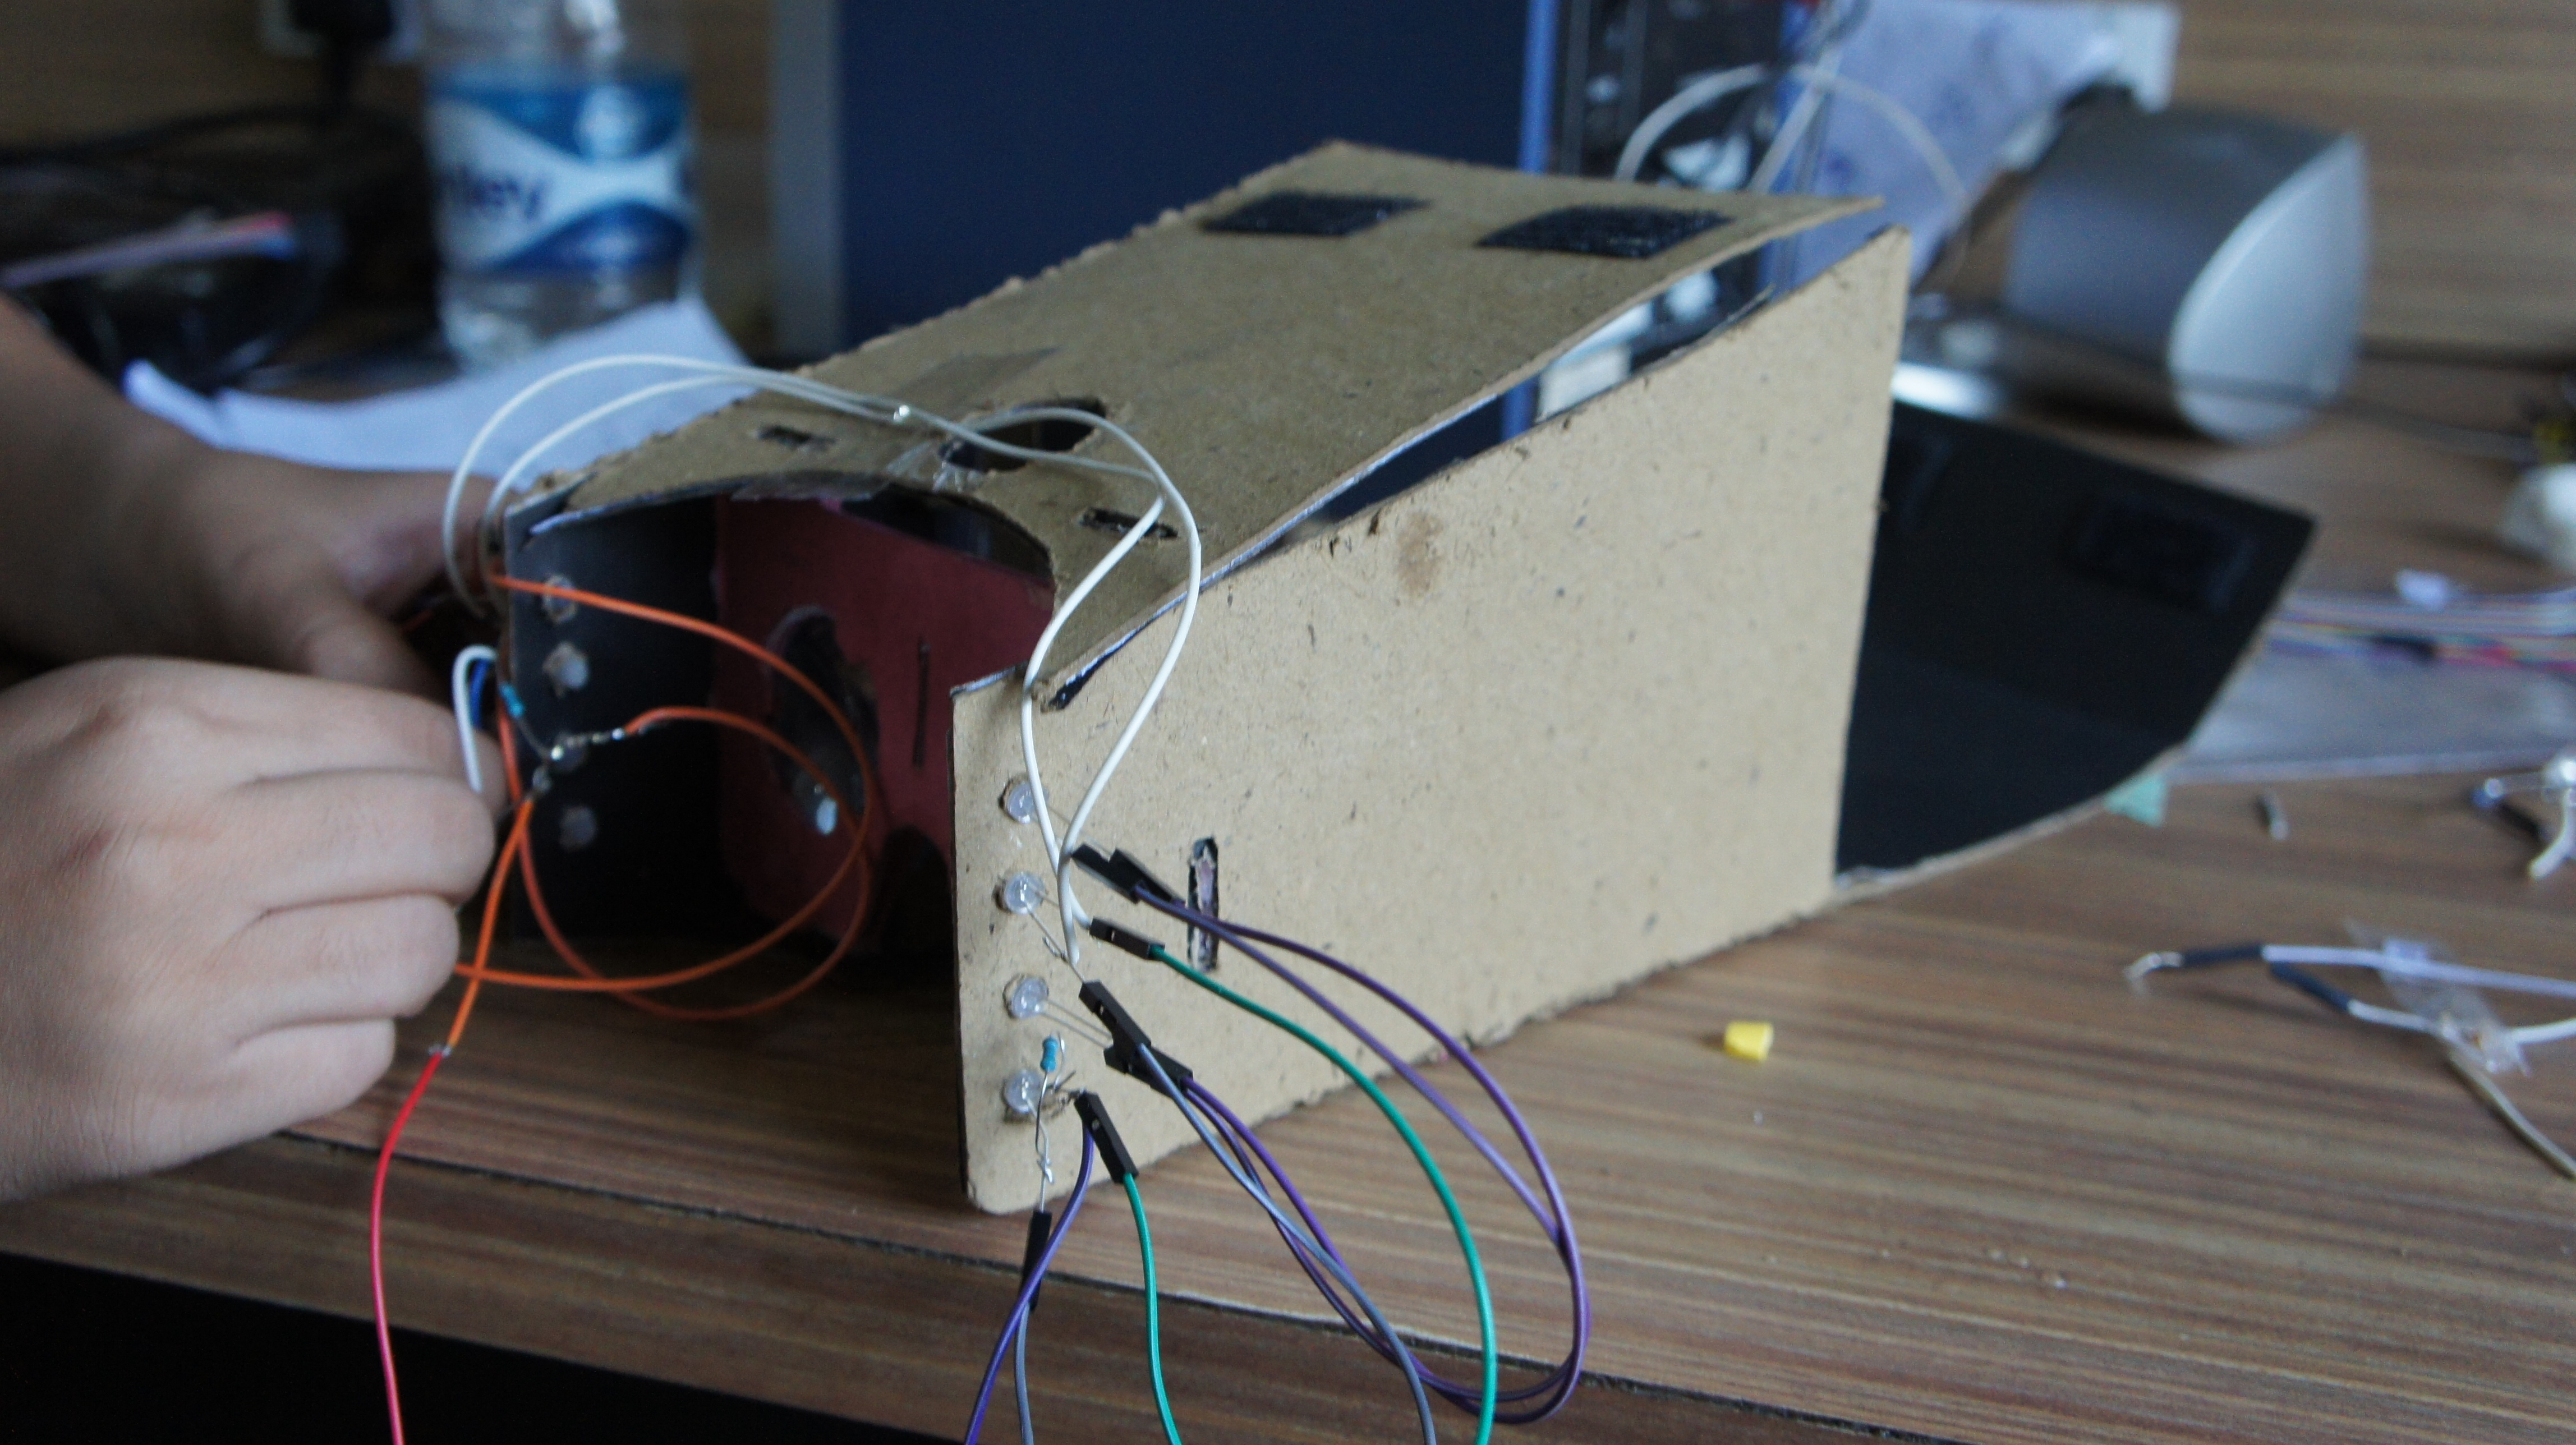
\includegraphics[width=8cm]{DSC03895} 
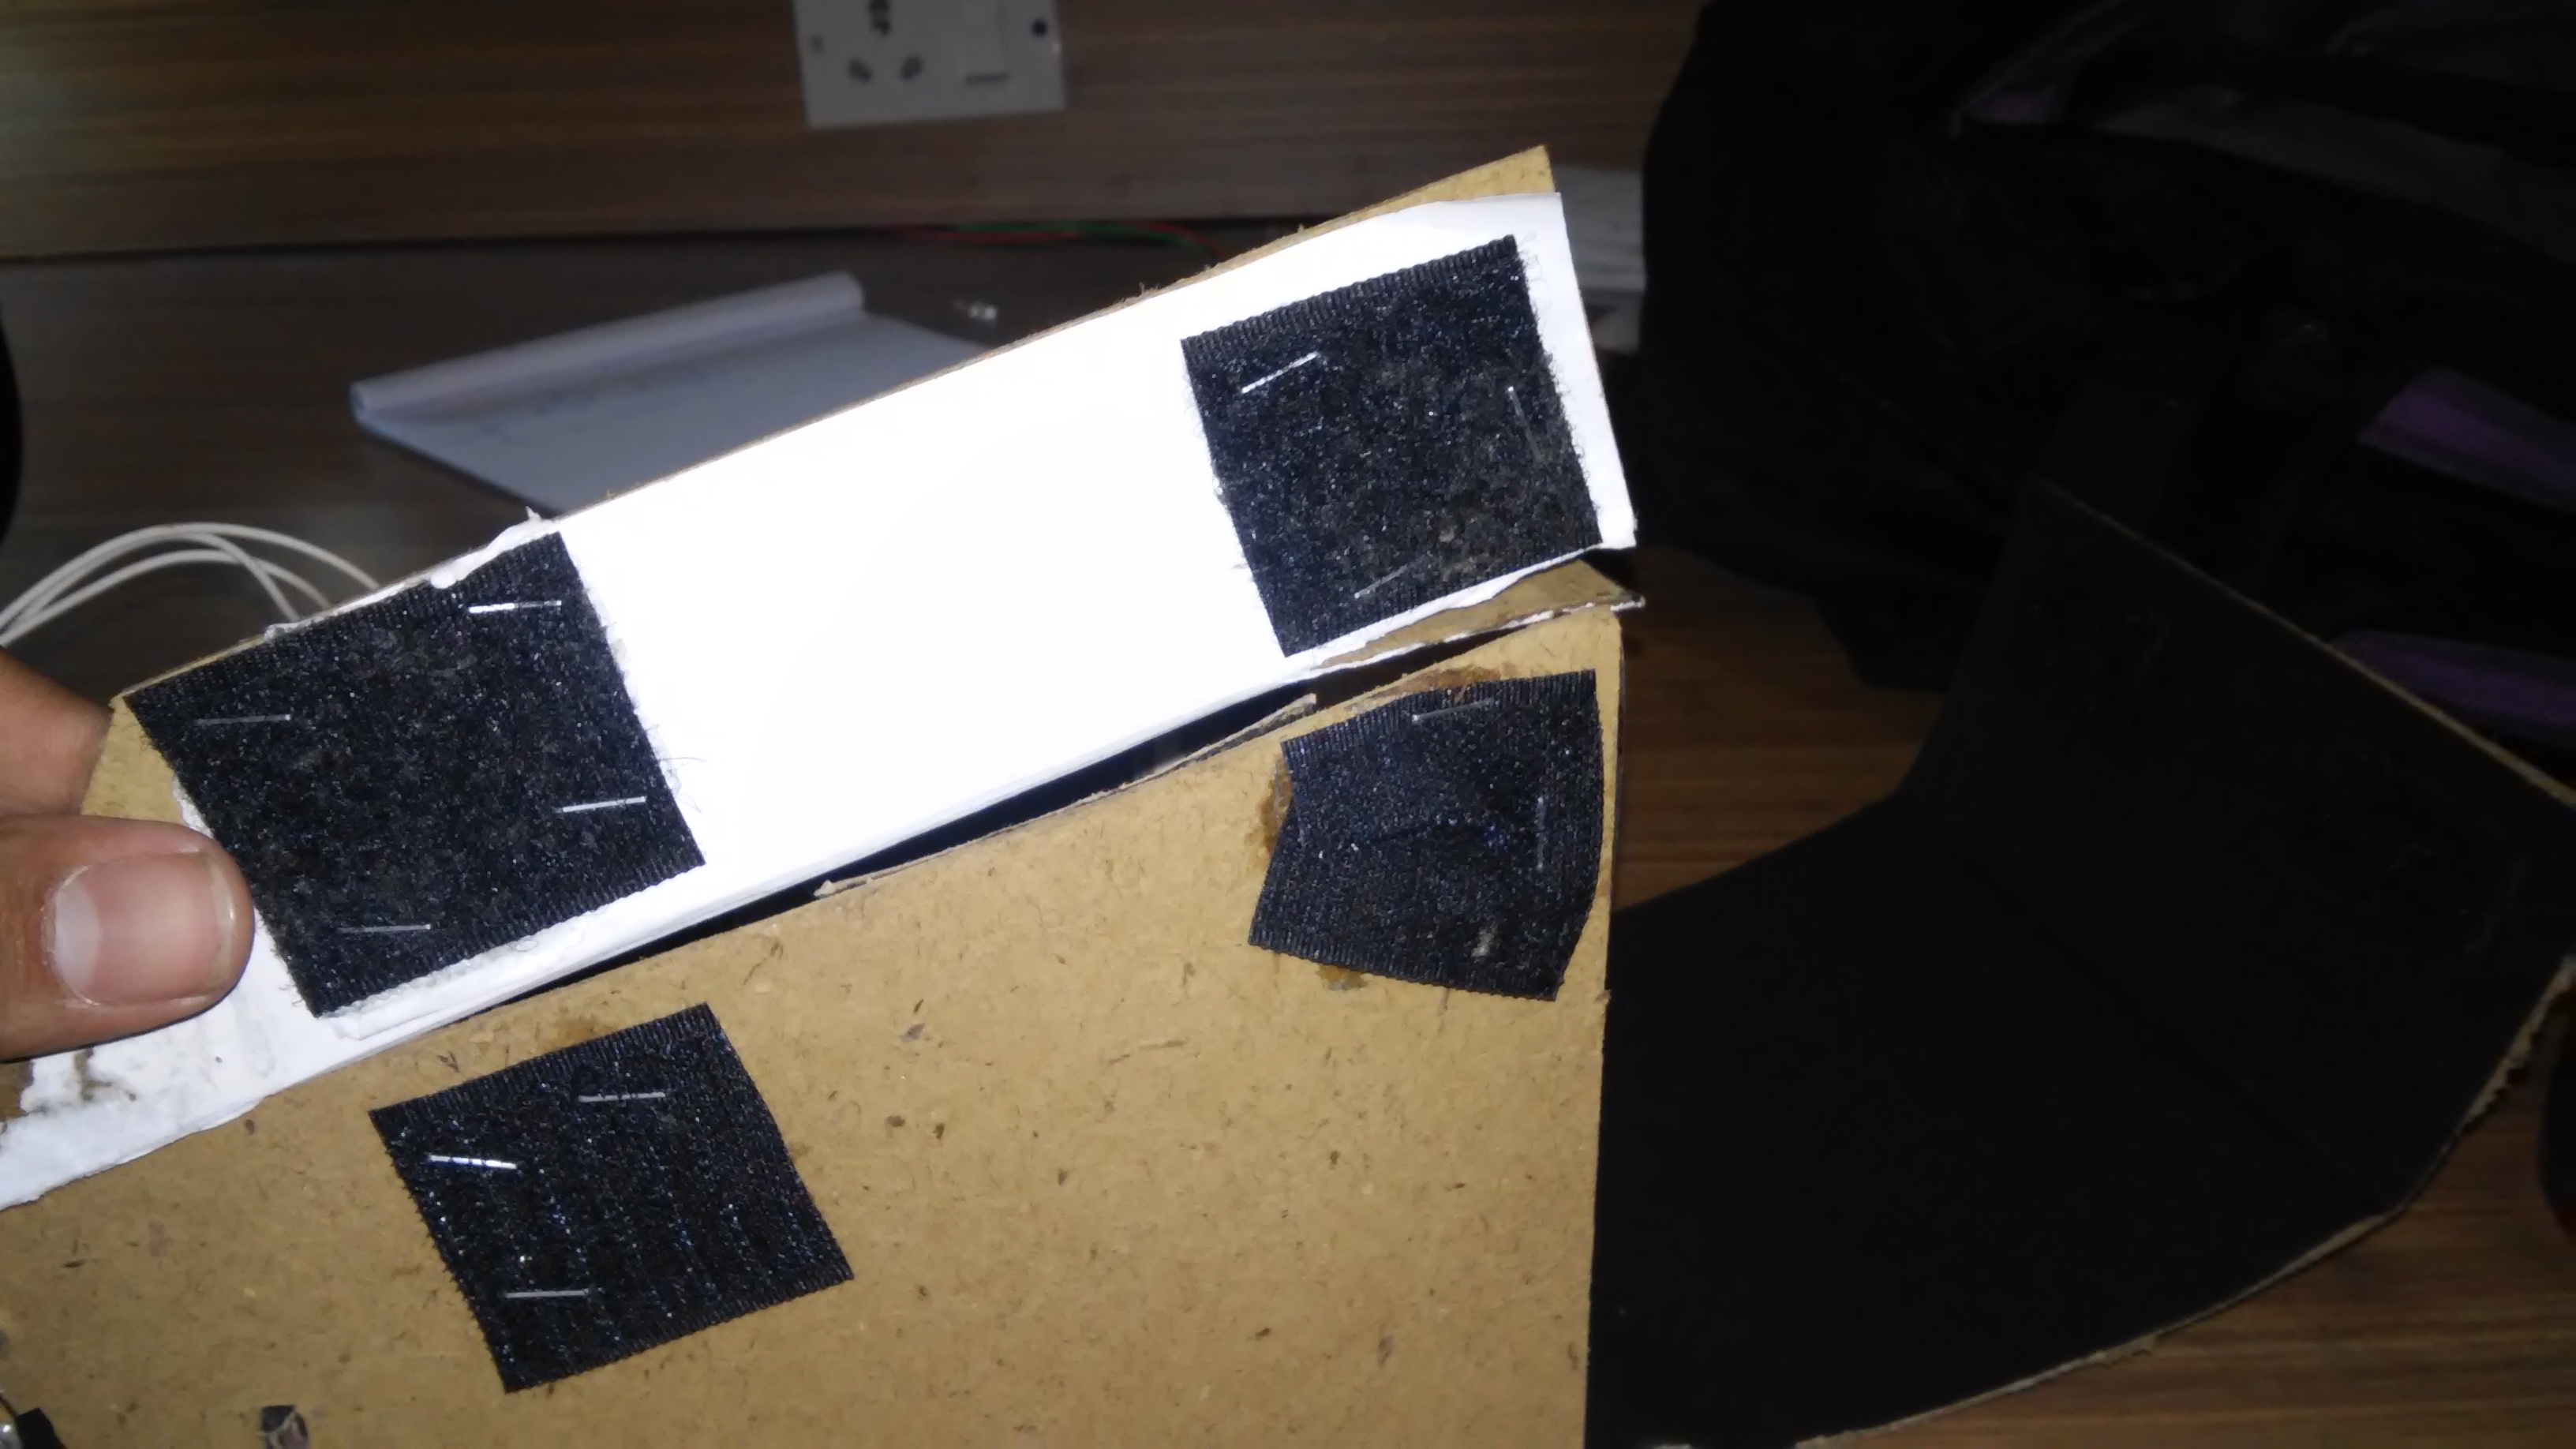
\includegraphics[width=8cm]{20141225_162318} 


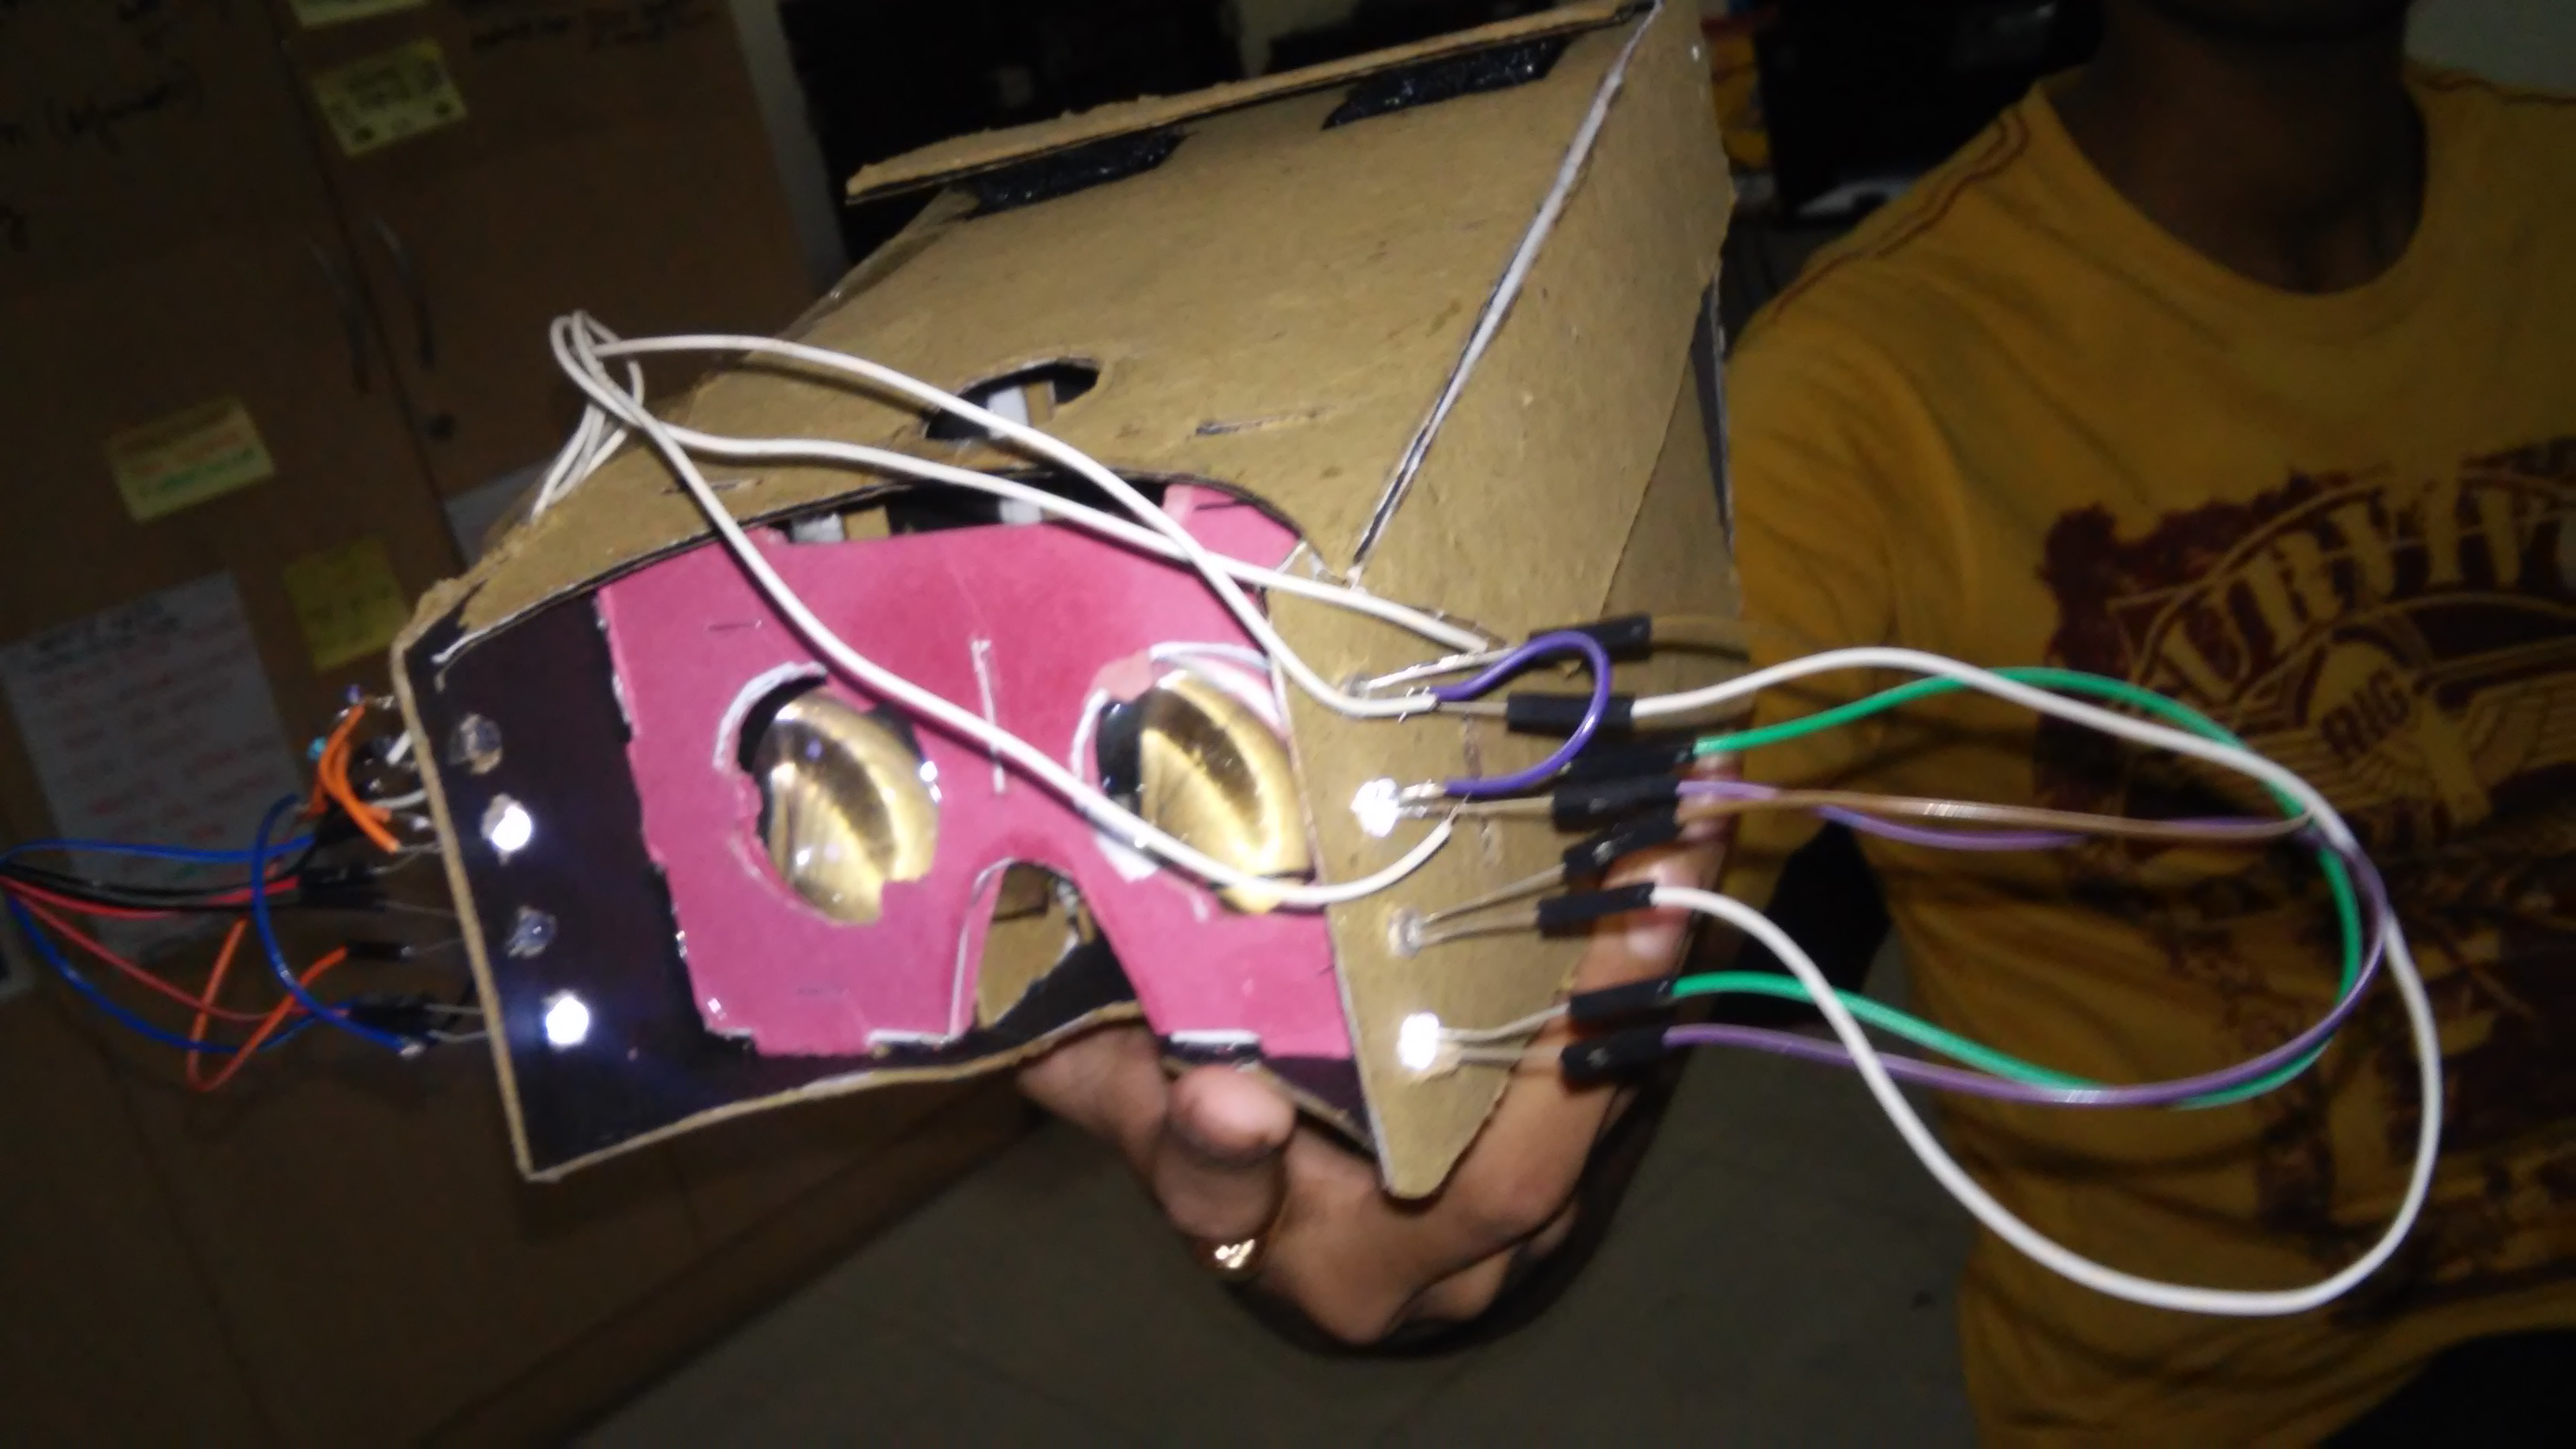
\includegraphics[width=8cm]{20141225_172947} 
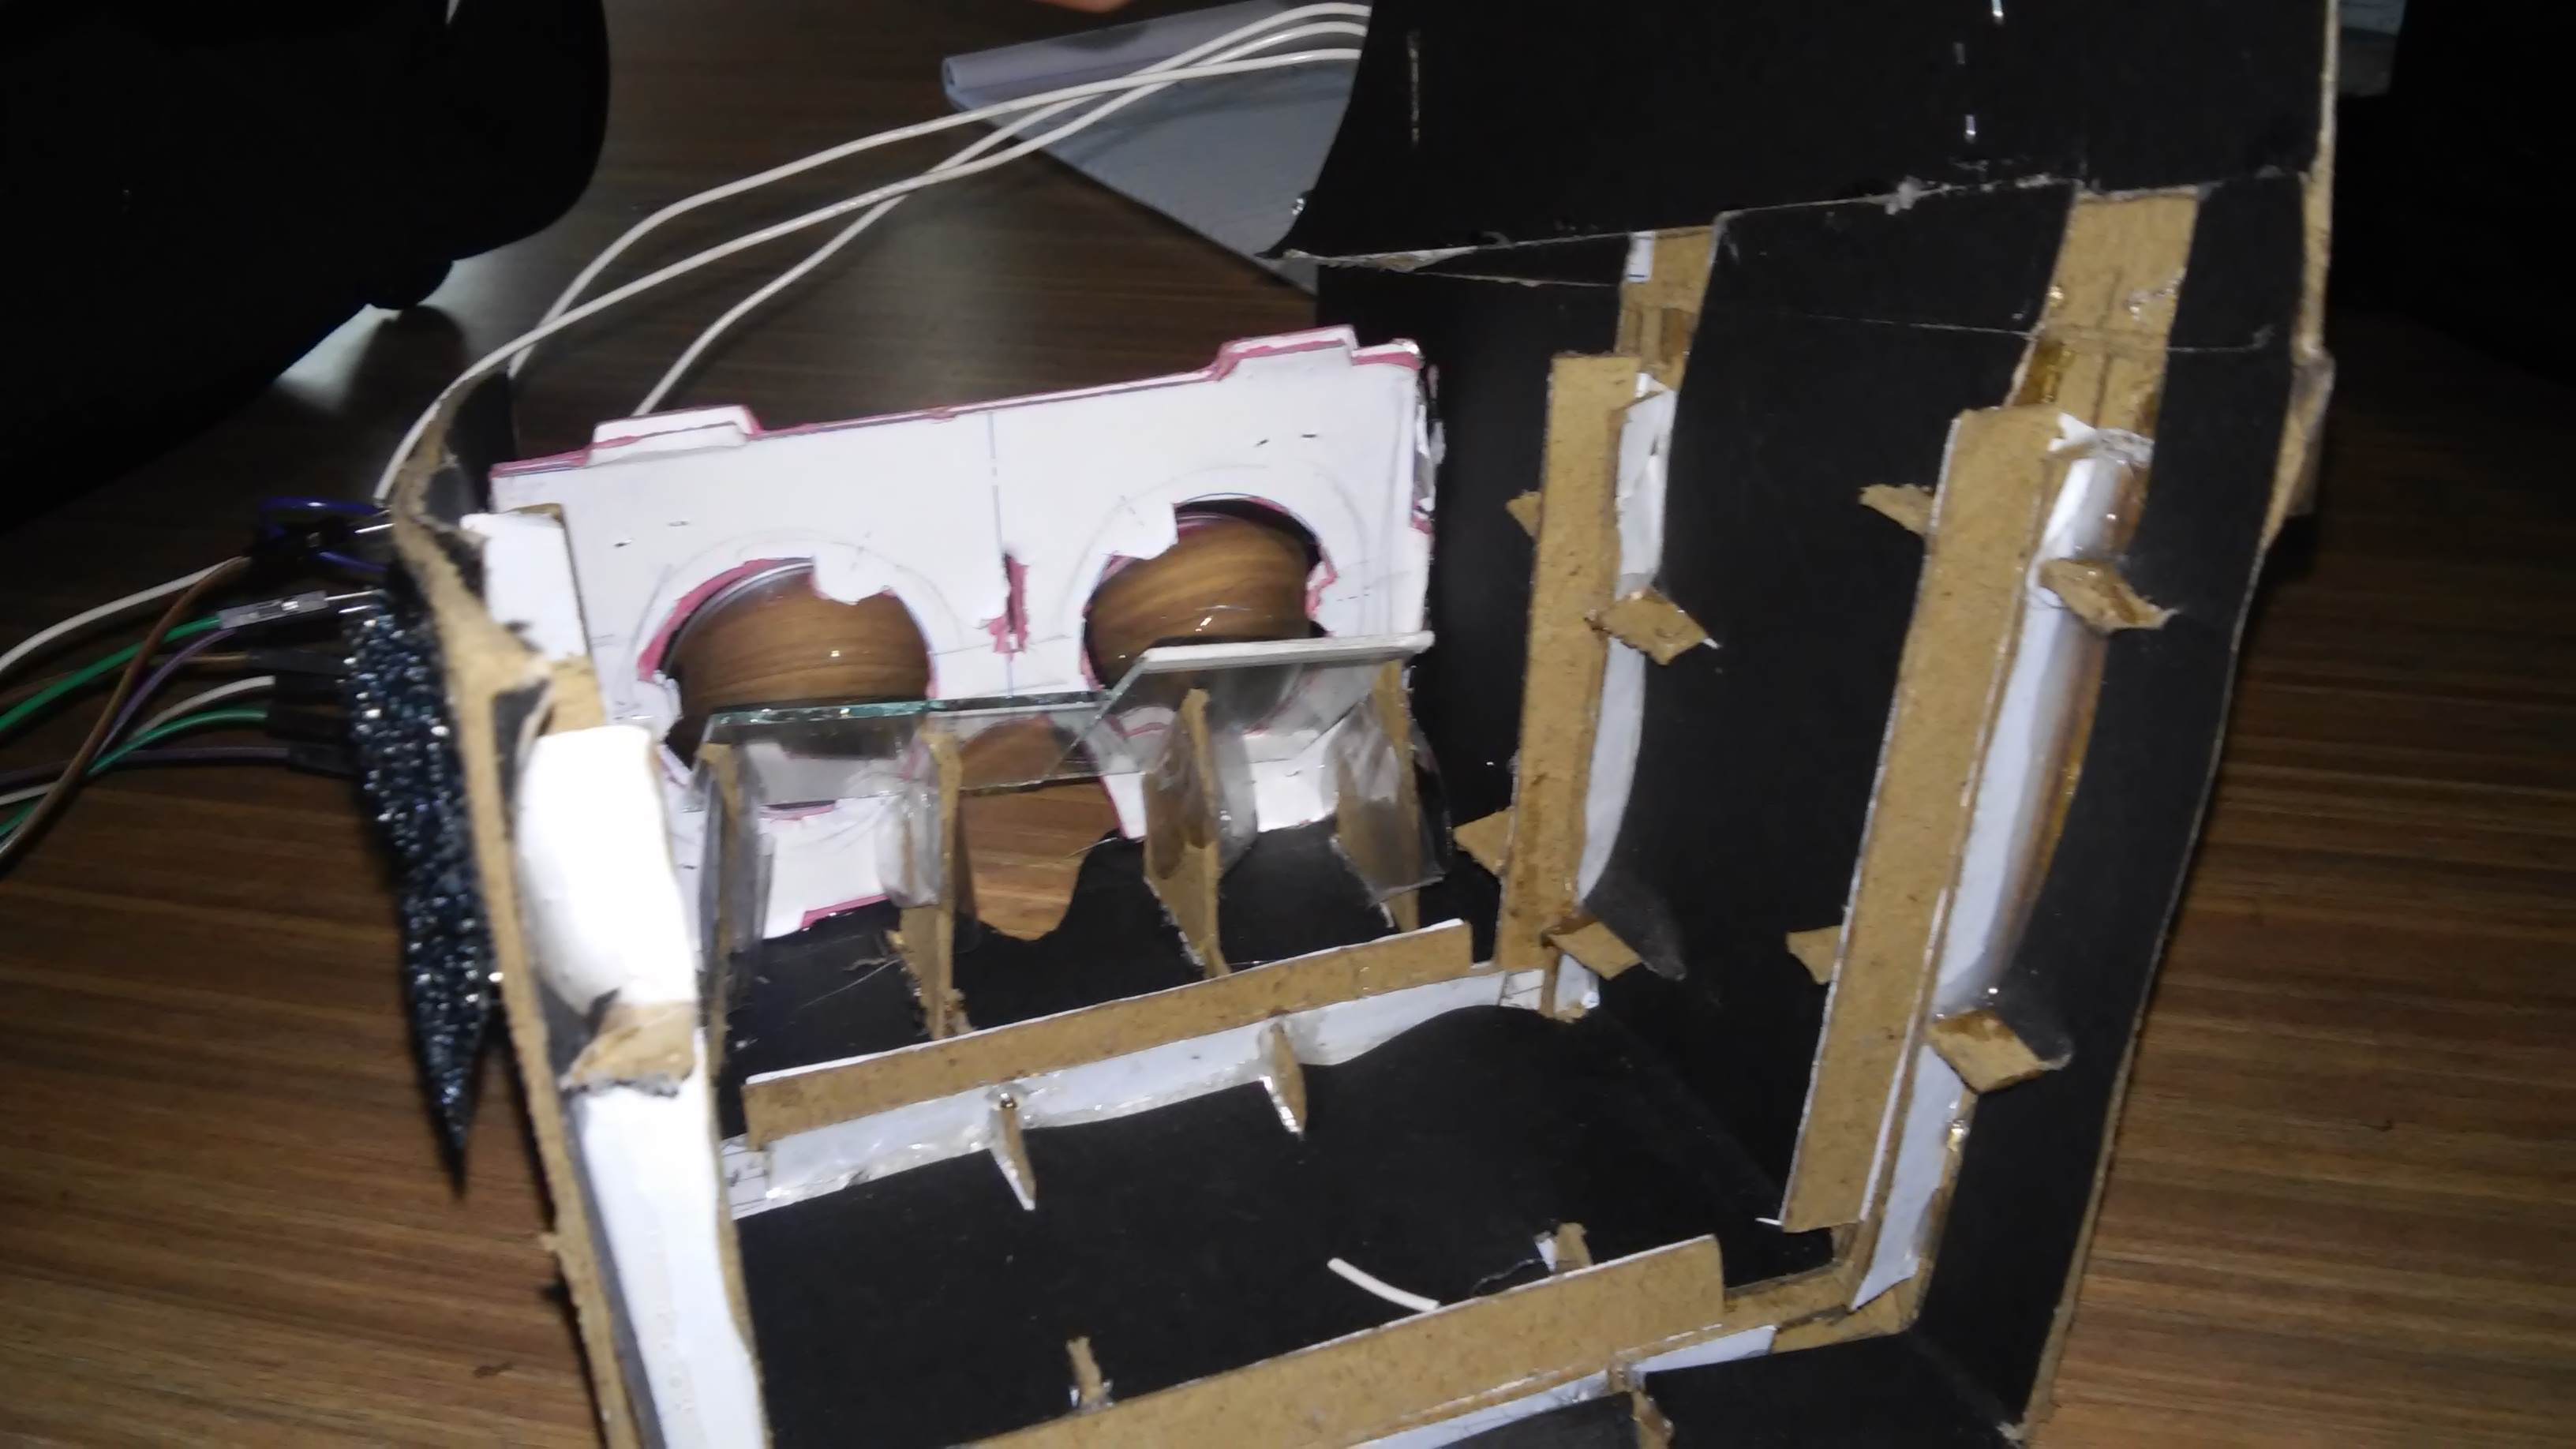
\includegraphics[width=8cm]{20141225_162310} \\


This prototype uses lens of focal length 5.5cm, and has two slots for fitting in LCDs. We have fitted 2 White LEDs and 2 IR LEDs altenatively on each side. The inside of box is covered with black chart paper so that no reflections are obtained.A camera is attached at the top  and 2 beam splitters are fixed at the base which are inclined at angle of 45 degree. It is a box which can be opened from upper surface (as shown in figure, using velcro) which allows us to inspect and experiment the inside of the box properly, the fitting of beam splitters, camera with proper alignment. \\
A  9V battery, 2 560 ohms, 2 330 ohm resistors, 8 LEDS are fixed as shown as figure.\\
 

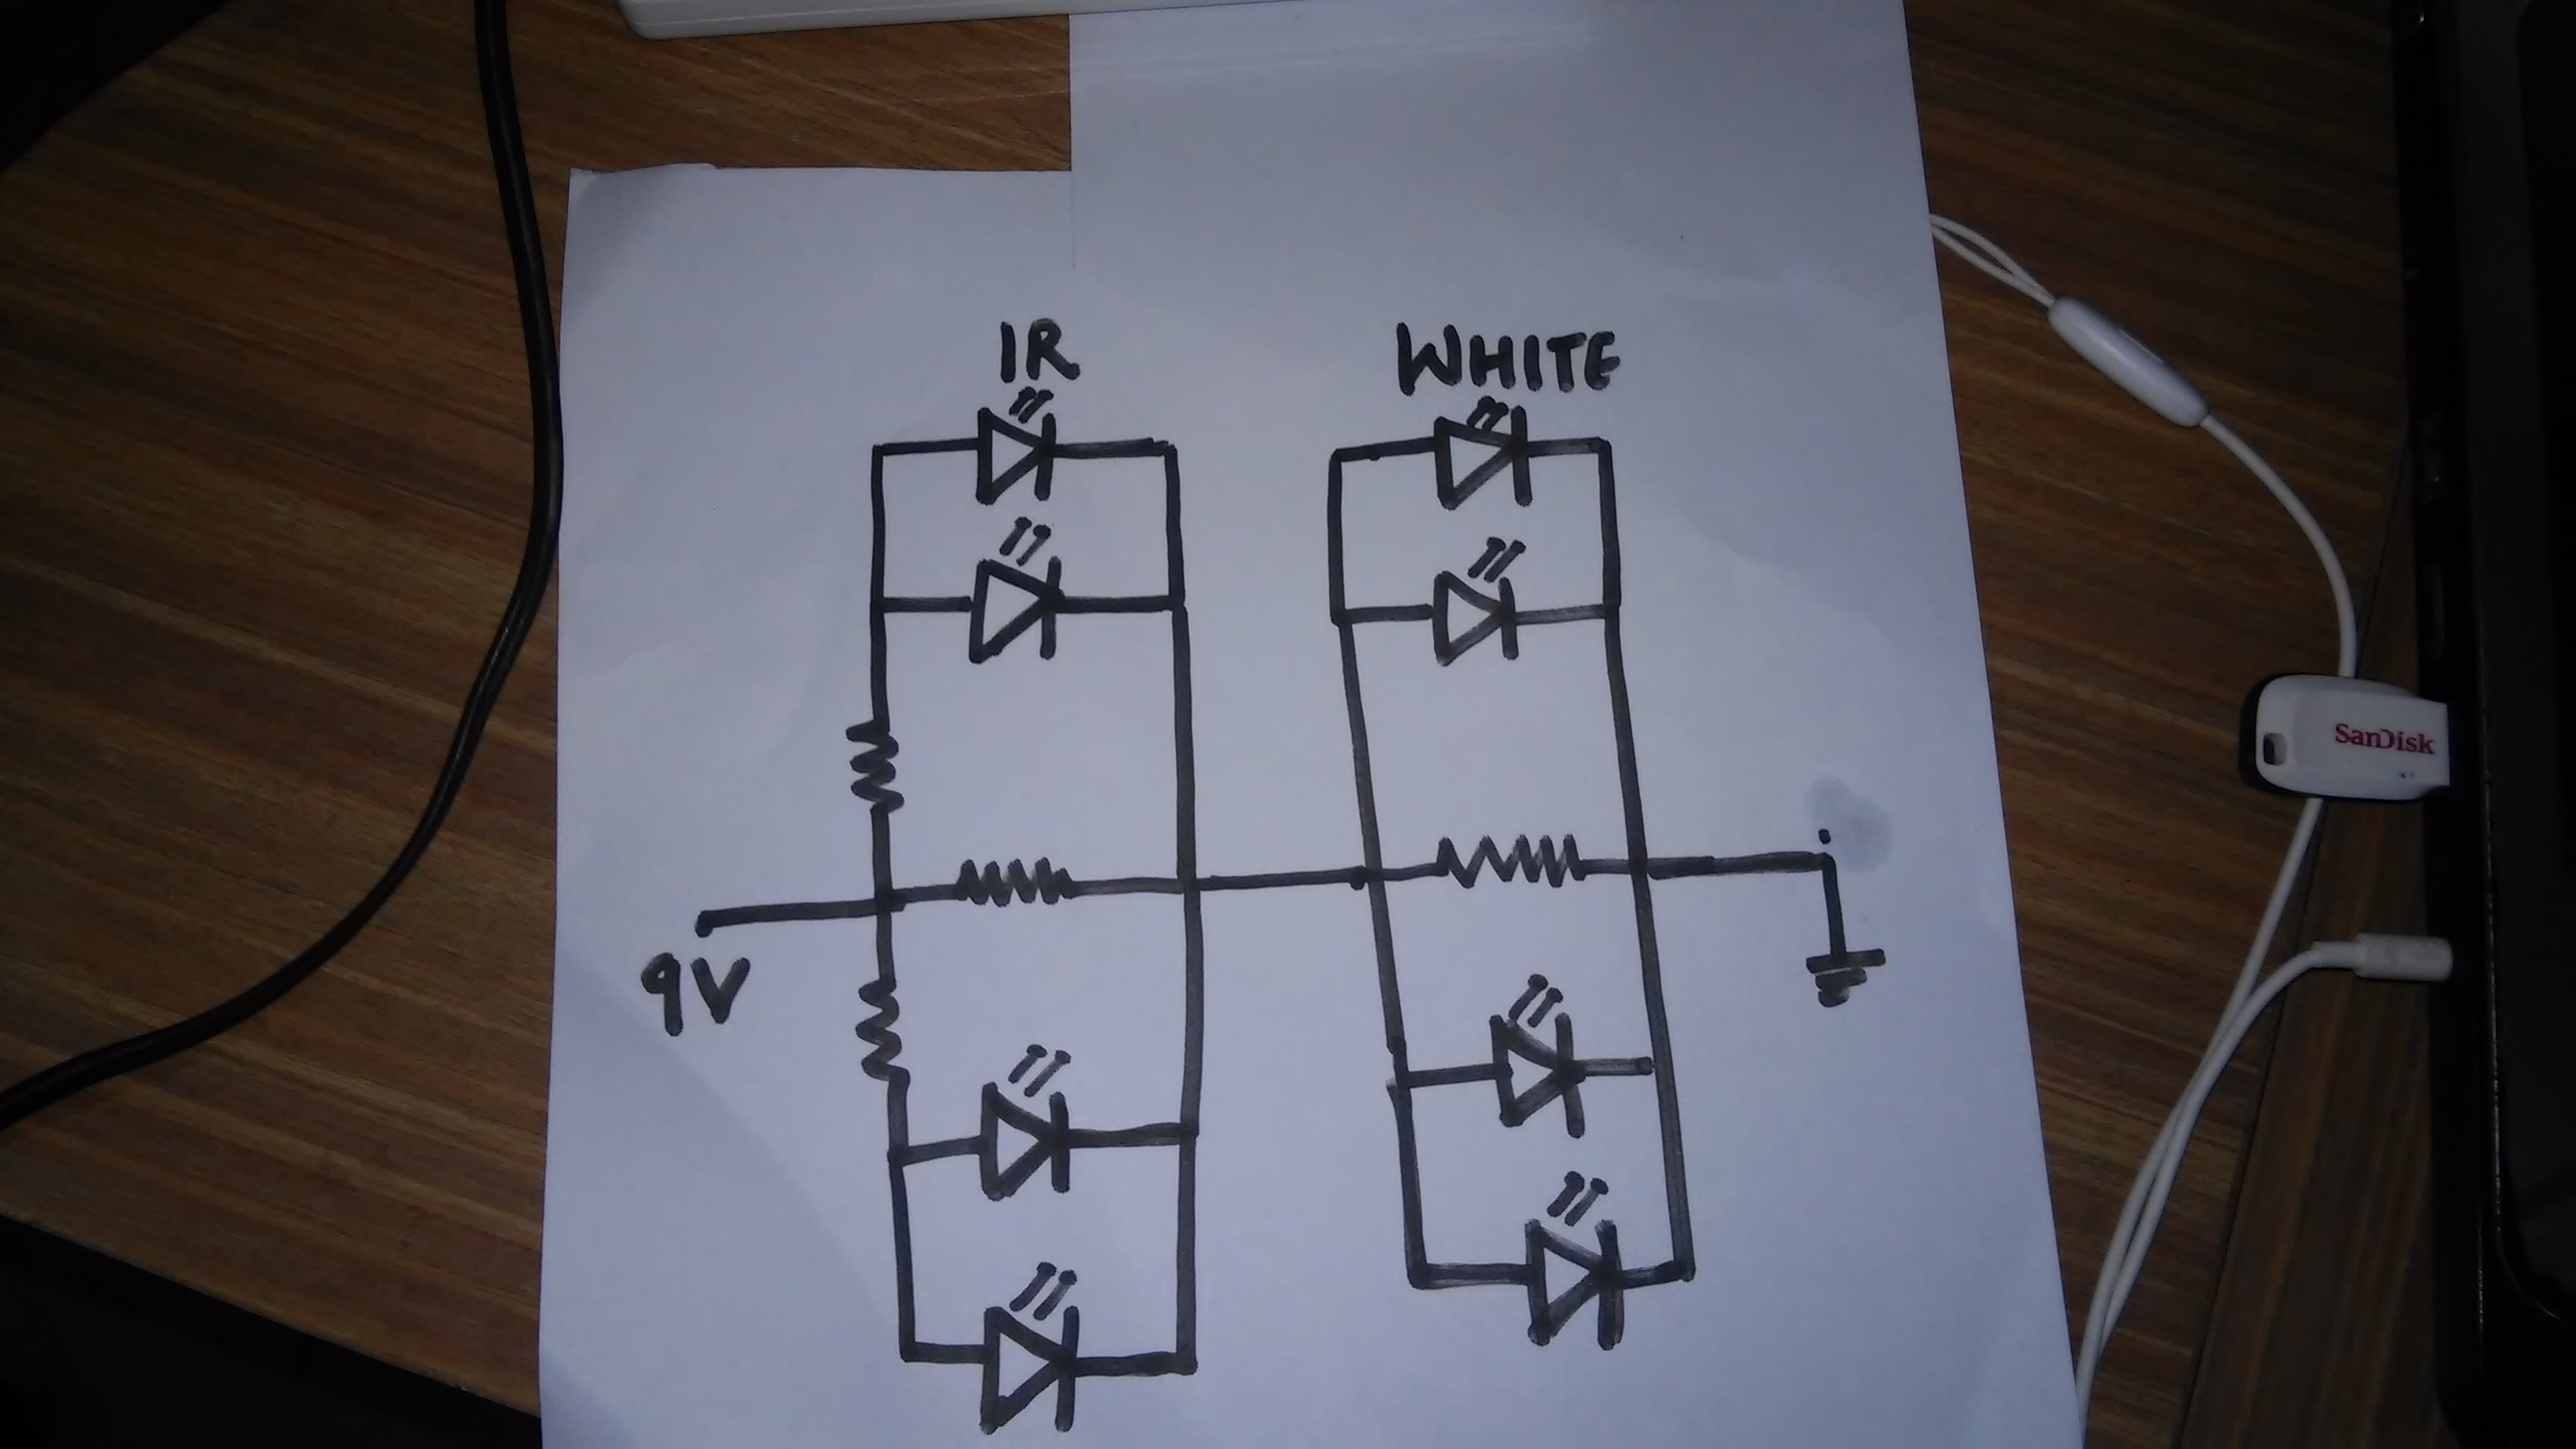
\includegraphics[width=8cm]{20141225_171833}
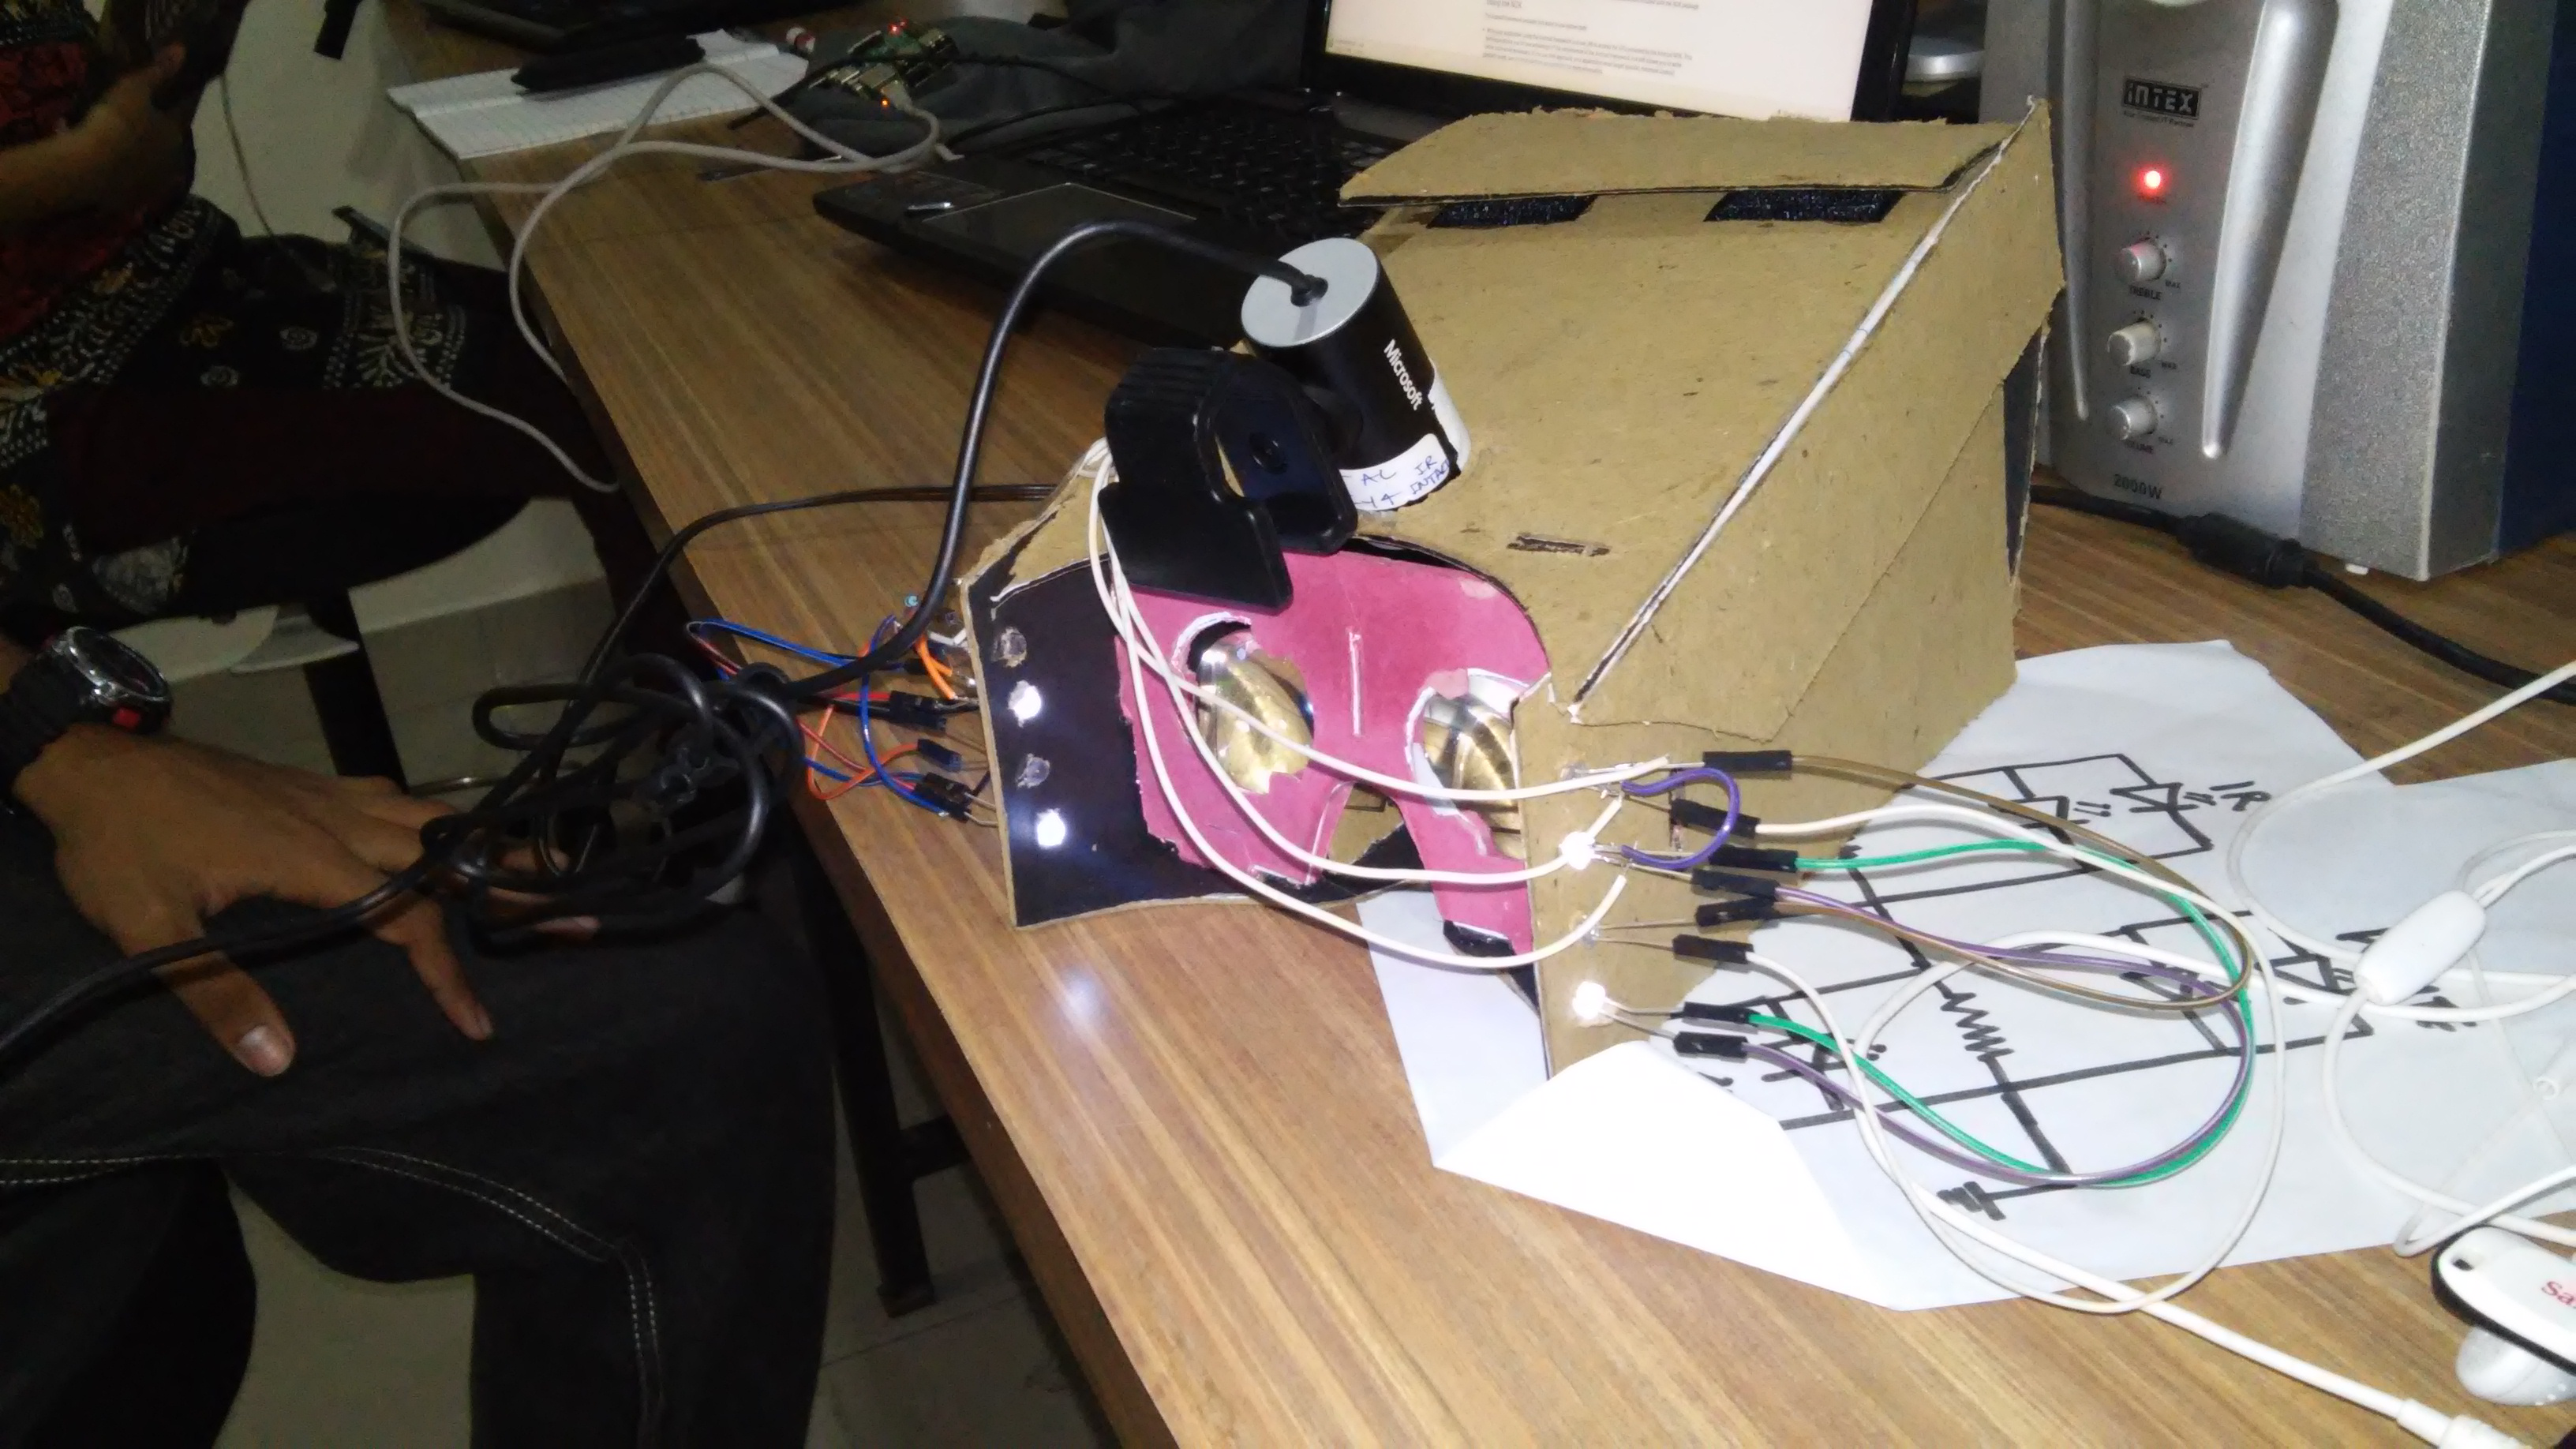
\includegraphics[width=8cm]{20141225_173411} 


 \subsection{Image Processing using C++'s OpenCV Library}

I tried my hands on image processing using C++'s OpenCV Library. I tried to implement different kinds of processing techniques like blurring, edge detection onto an image along with different types of techniques like Guassian Blur, Adaptive thresholding, median Blur, Canny Edge detection, sobel operator, Laplacian operator etc. The importance of this GUI software is that any image can be processed according to user's choice amongst all the functions and techniques available. \\


\begin{figure}[h!]
  \caption{Creating trackbars in different windows: }
  \centering
 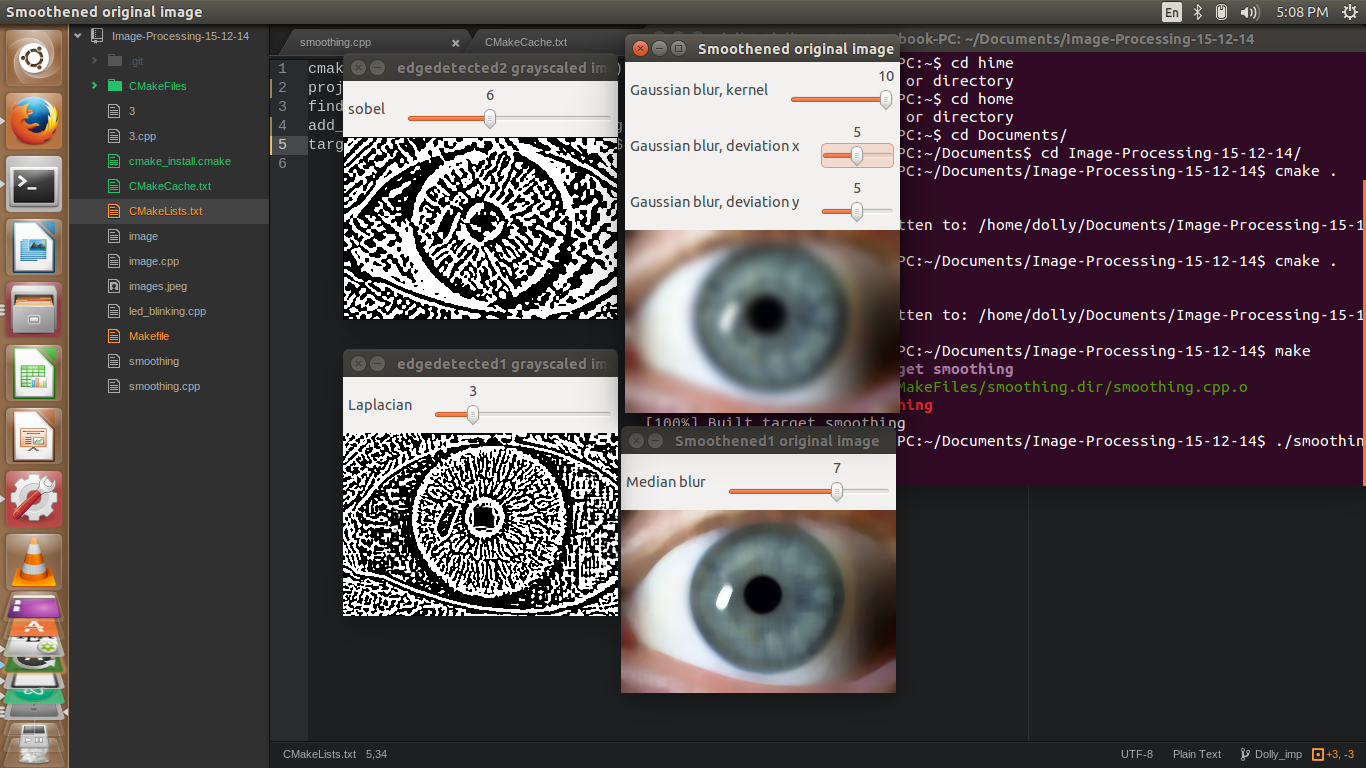
\includegraphics[width=8cm]{img.png}\\
 \end{figure}
The code can be found here:\\

\url{<https://github.com/deveshjain94/Image-Processing-15-12-14/blob/Dolly_imp/smoothing.cpp>}  

 \begin{figure}[h!]
  \caption{Combining all the trackbars into a single window: }
  \centering
 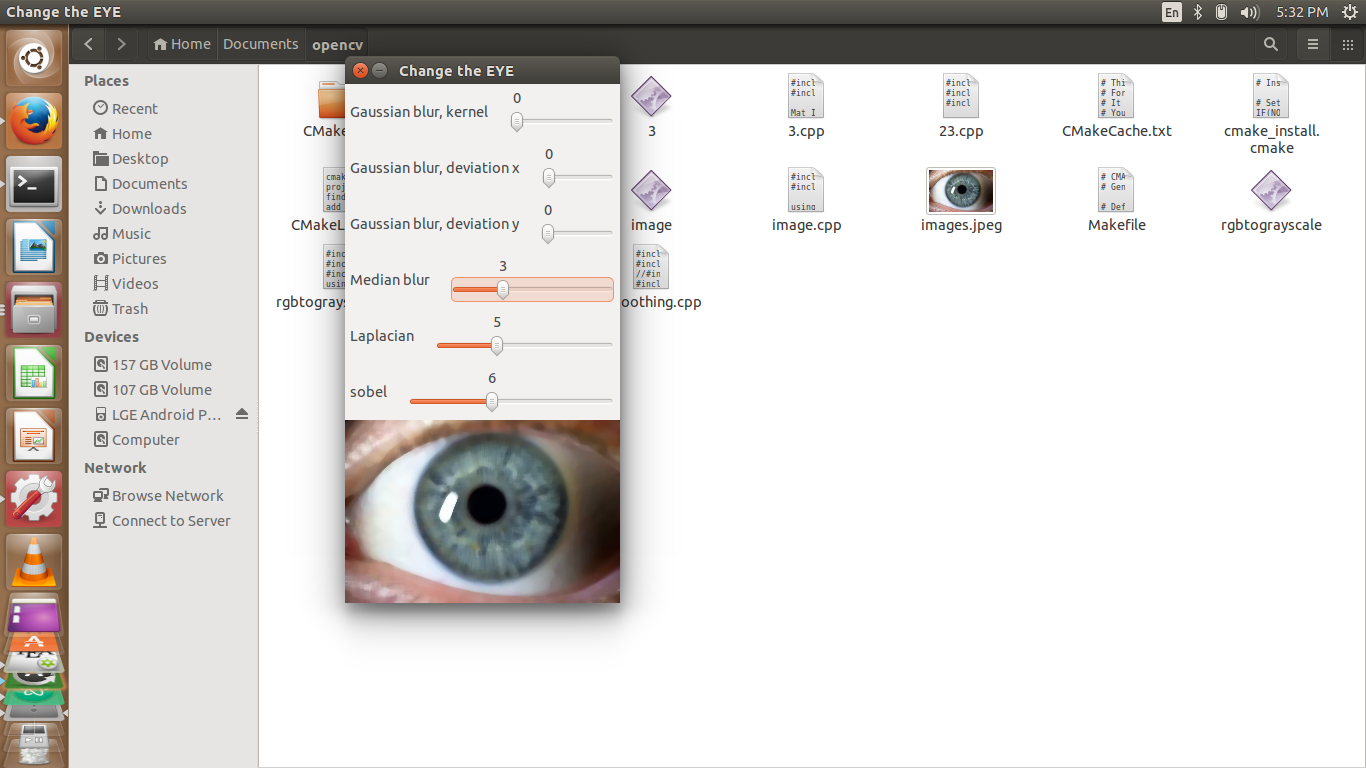
\includegraphics[width=8cm]{fe.png}
  \end{figure}
  
 \subsection{Corneal Topography}
1.)Working of corneal topographer: \\
-Non-invasive technique.
-A lighted bowl contains patterns of concentric rings. The patient is seated in front of the bowl, and placido rings are projected on to the cornea. 
-The camera takes a picture of a reflection. And a computer is used to analyse the distortions in reflections.
-The distortions are then printed on a colour coded map which are then printed out.
-The computer converts the ring spacing into a colour coded map. 

2.)Reflective image analysis:\\
  
This is the method of imaging of anterior segment of eye, uses the analysis of reflected images of multiple concentric rings projected onto the cornea.
Now I have projected a pattern of placido’s rings onto a curved surface. Now imaging of this surface will be done, (will consider this as anterior segment of eye). 
Second step is to form topographic map of this image obtained. For that I will convert this image into a grayscaled one, thresholded one. 
These topographic colour coded maps are formed by first determining the keratometric Diopter values.
Each colour is assigned one diopteric range.
Power map/curvature map:
Elevation map: elevation of  a corneal surface from a certain reference height.
An absolute scale is used which states the center point as 45D and evenly distribute the colours across the scale.

Analysis steps:\\
Take images from videokeratometer. (Videokeratography is a common method used by clinicians and researchers to estimate the surface topography of the human cornea. It is based on the object-to-image relationship of concentric rings reflected off the surface of the cornea. )
Running an algorithm to recover some aspects of corneal shape.
Outputting this information for analysis and further display. 

Normal algorithms from videokeratographs take the reflected ray from non-principal meridian axis to lie on the same plane, which generates errors. The ray leaving from such axes are skewed and hence no longer remains in the same plane as object ray.  This error can be corrected by analysing all the corneal points to a complex surface.

We tried to project the image of placido's ring by making a hardware design which is designed in a manner that accomodates a camera in center which takes the image reflected from the corneal surface.\\

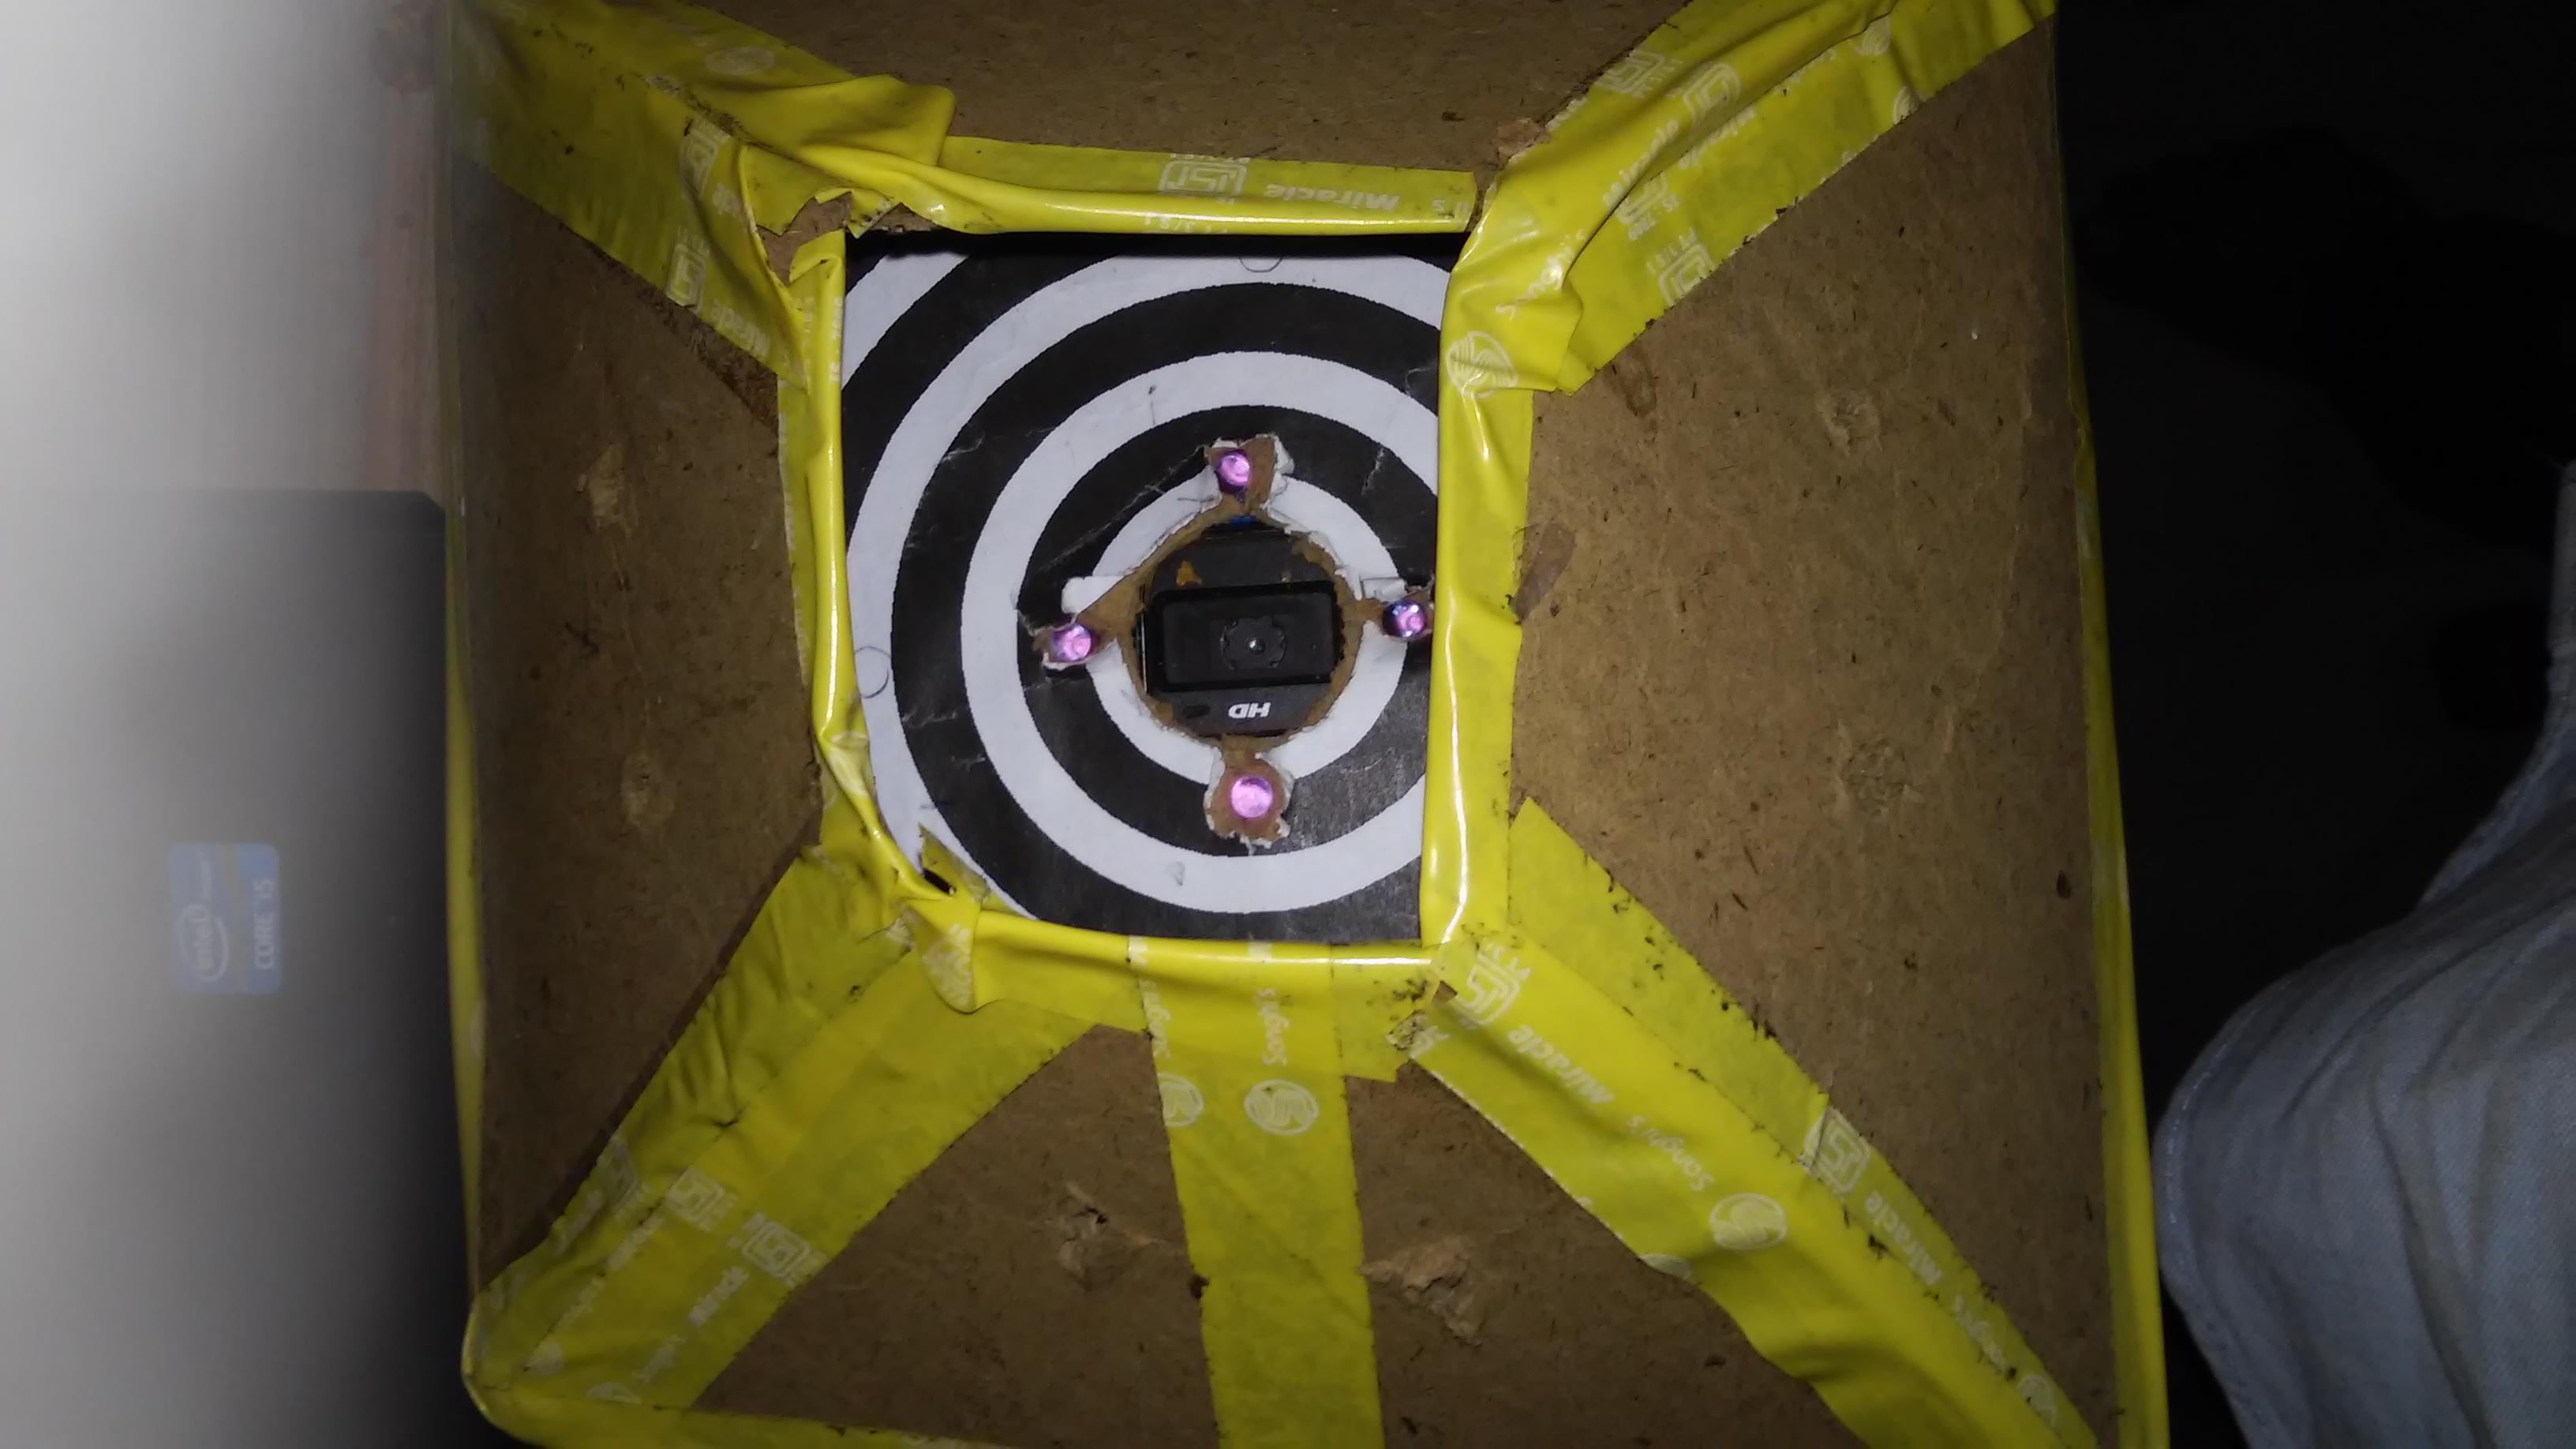
\includegraphics[width=5cm]{rr.jpg}
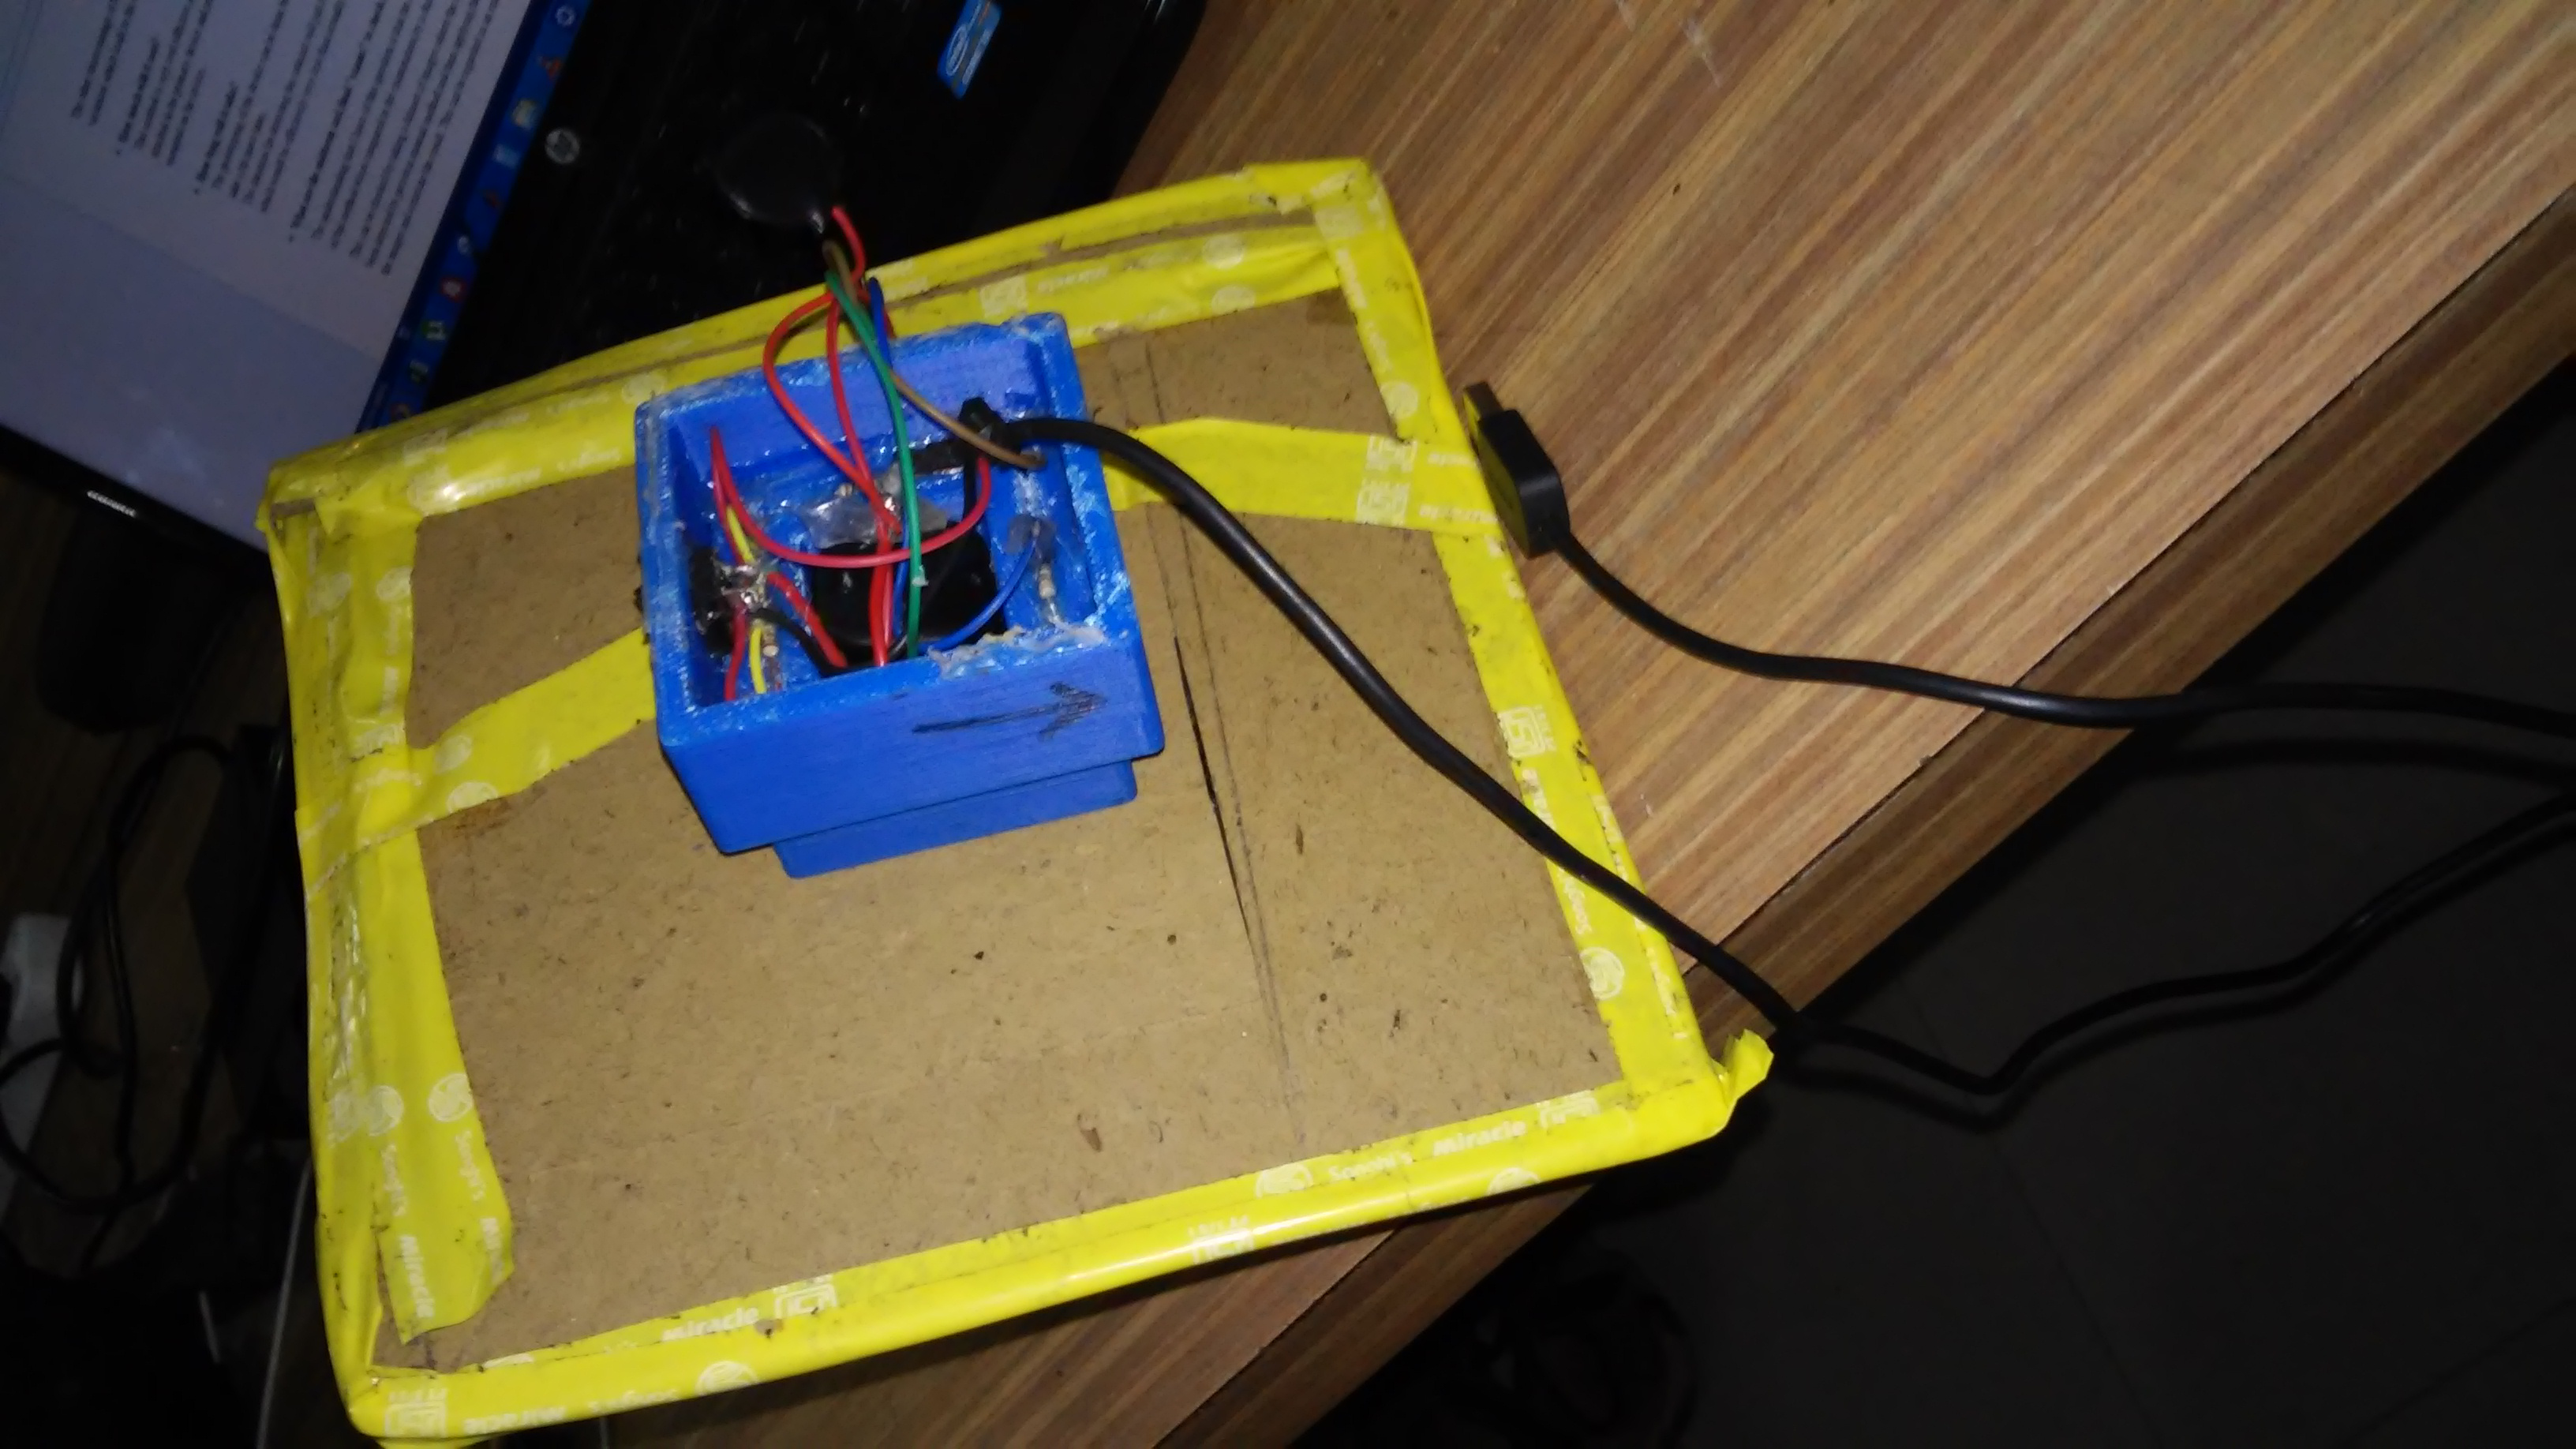
\includegraphics[width=5cm]{er.jpg}
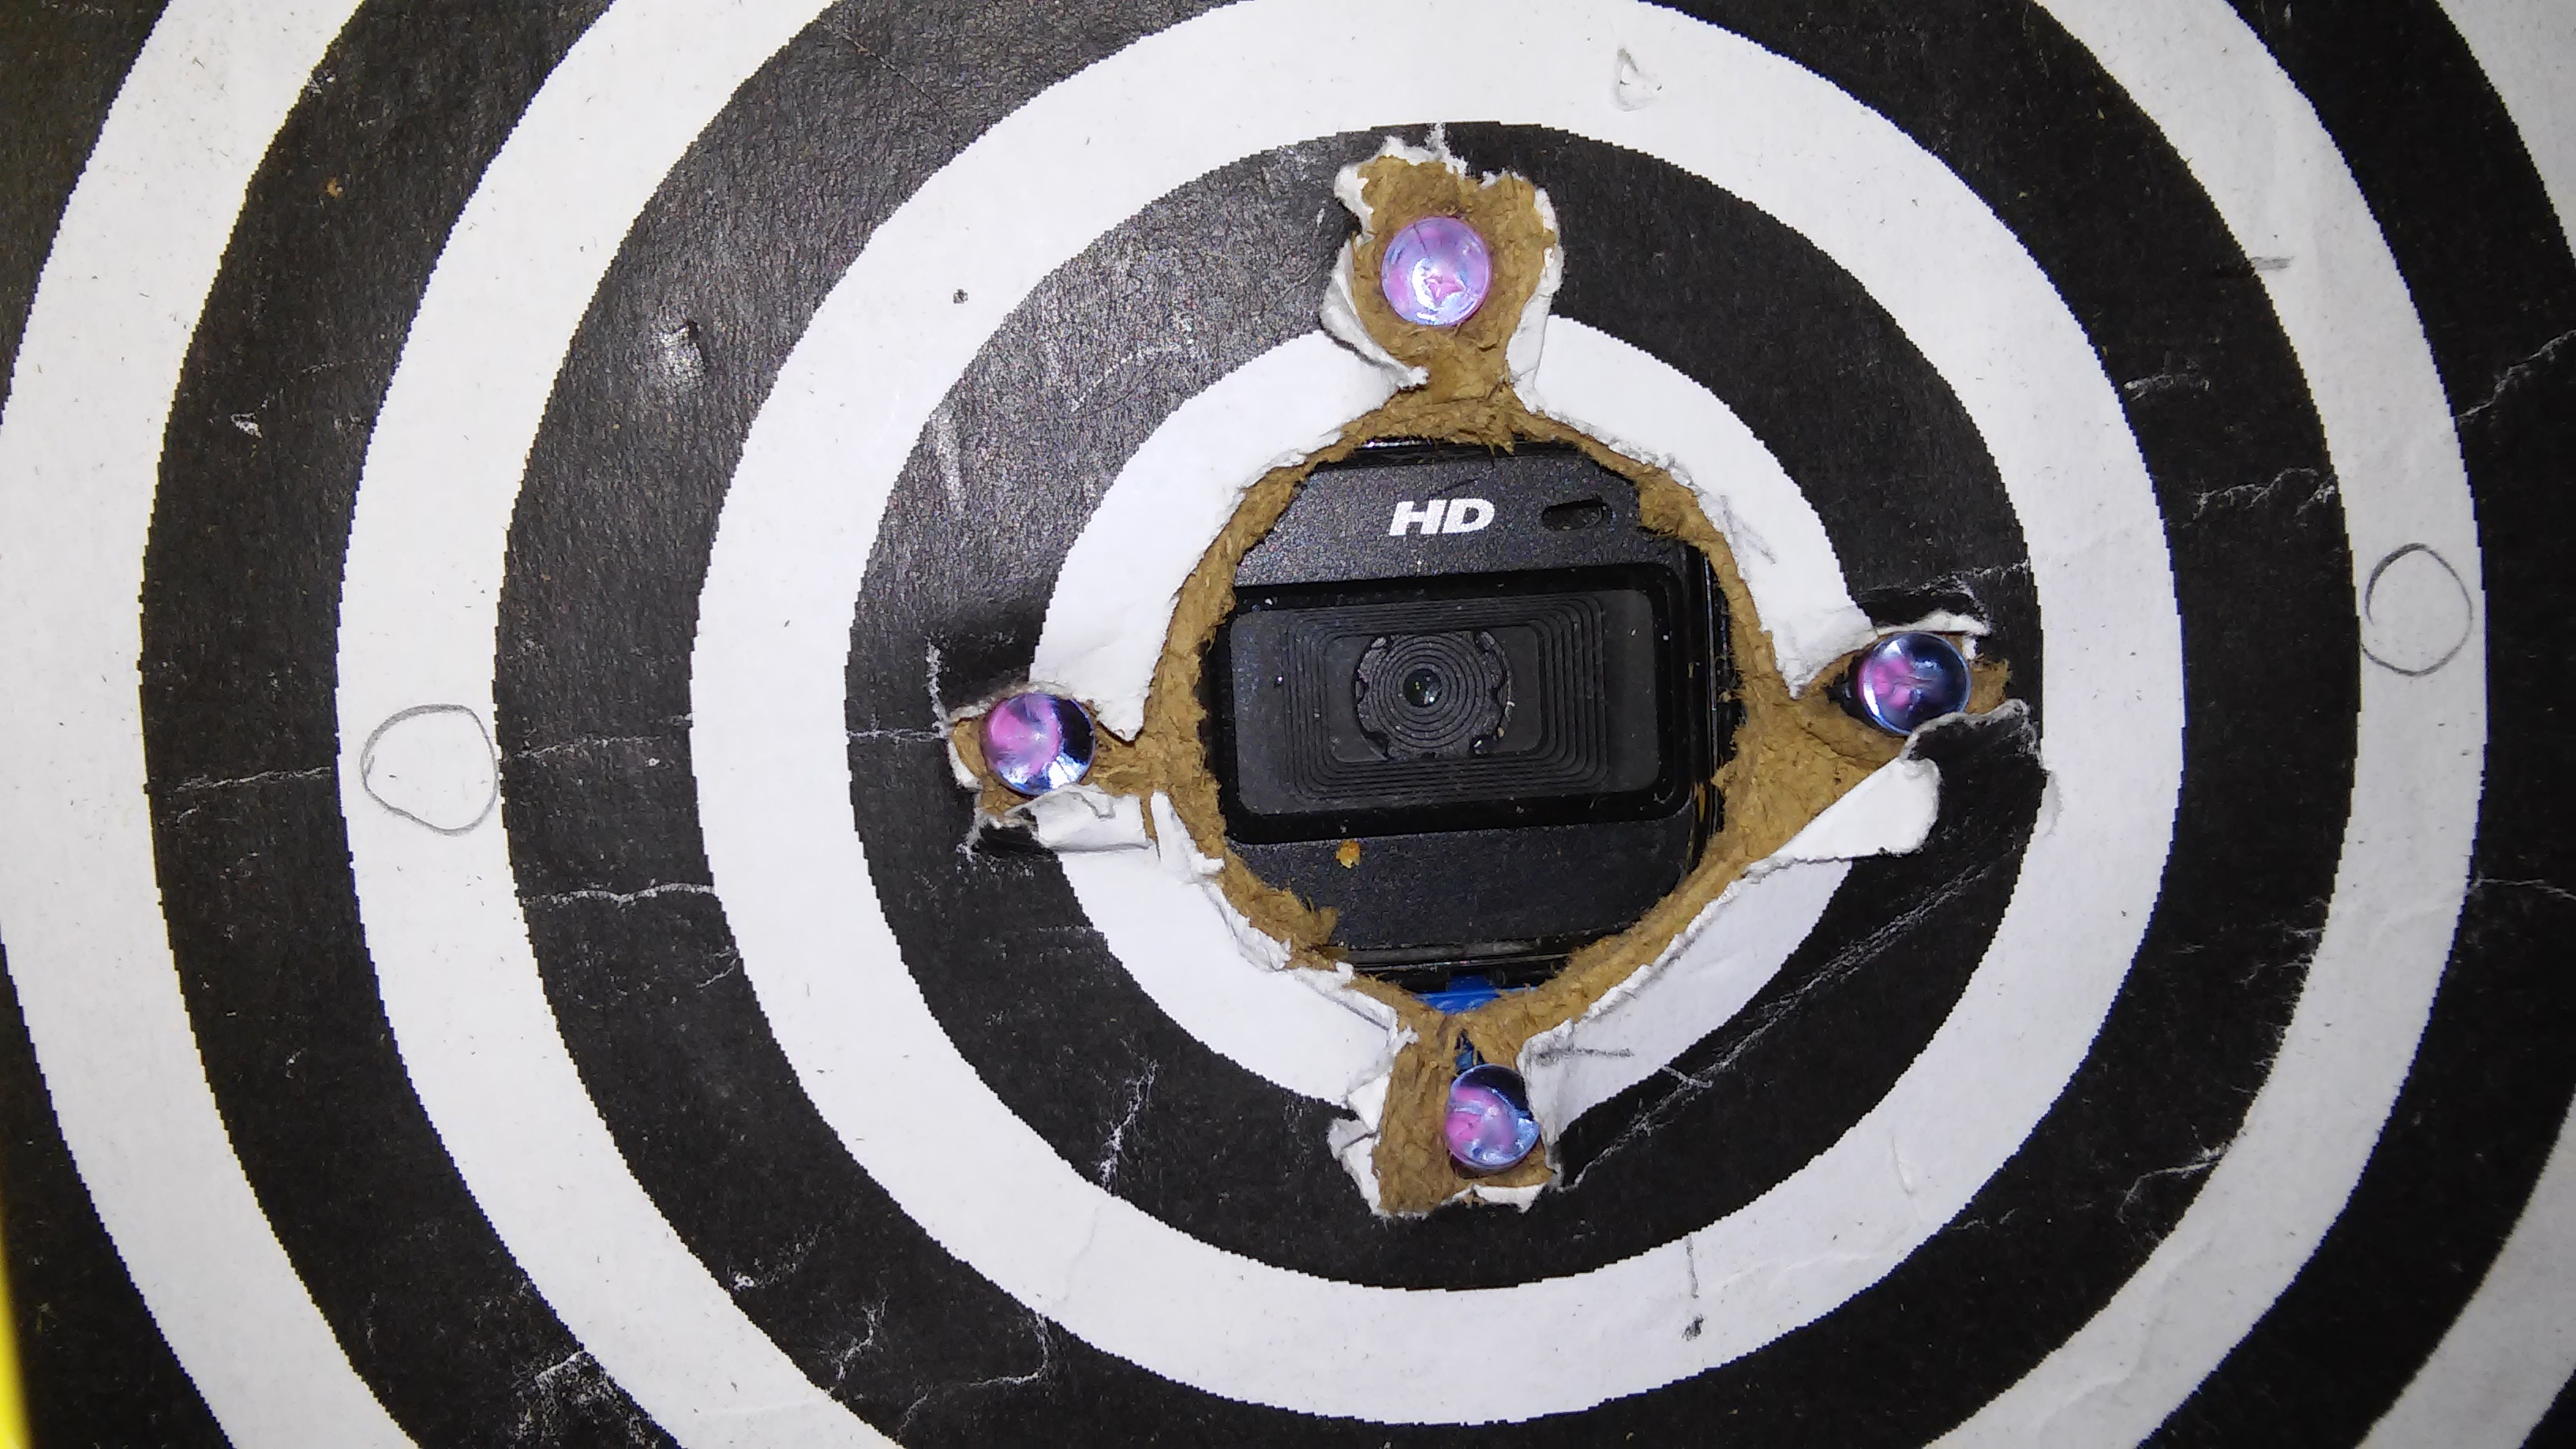
\includegraphics[width=5cm]{tr.jpg}

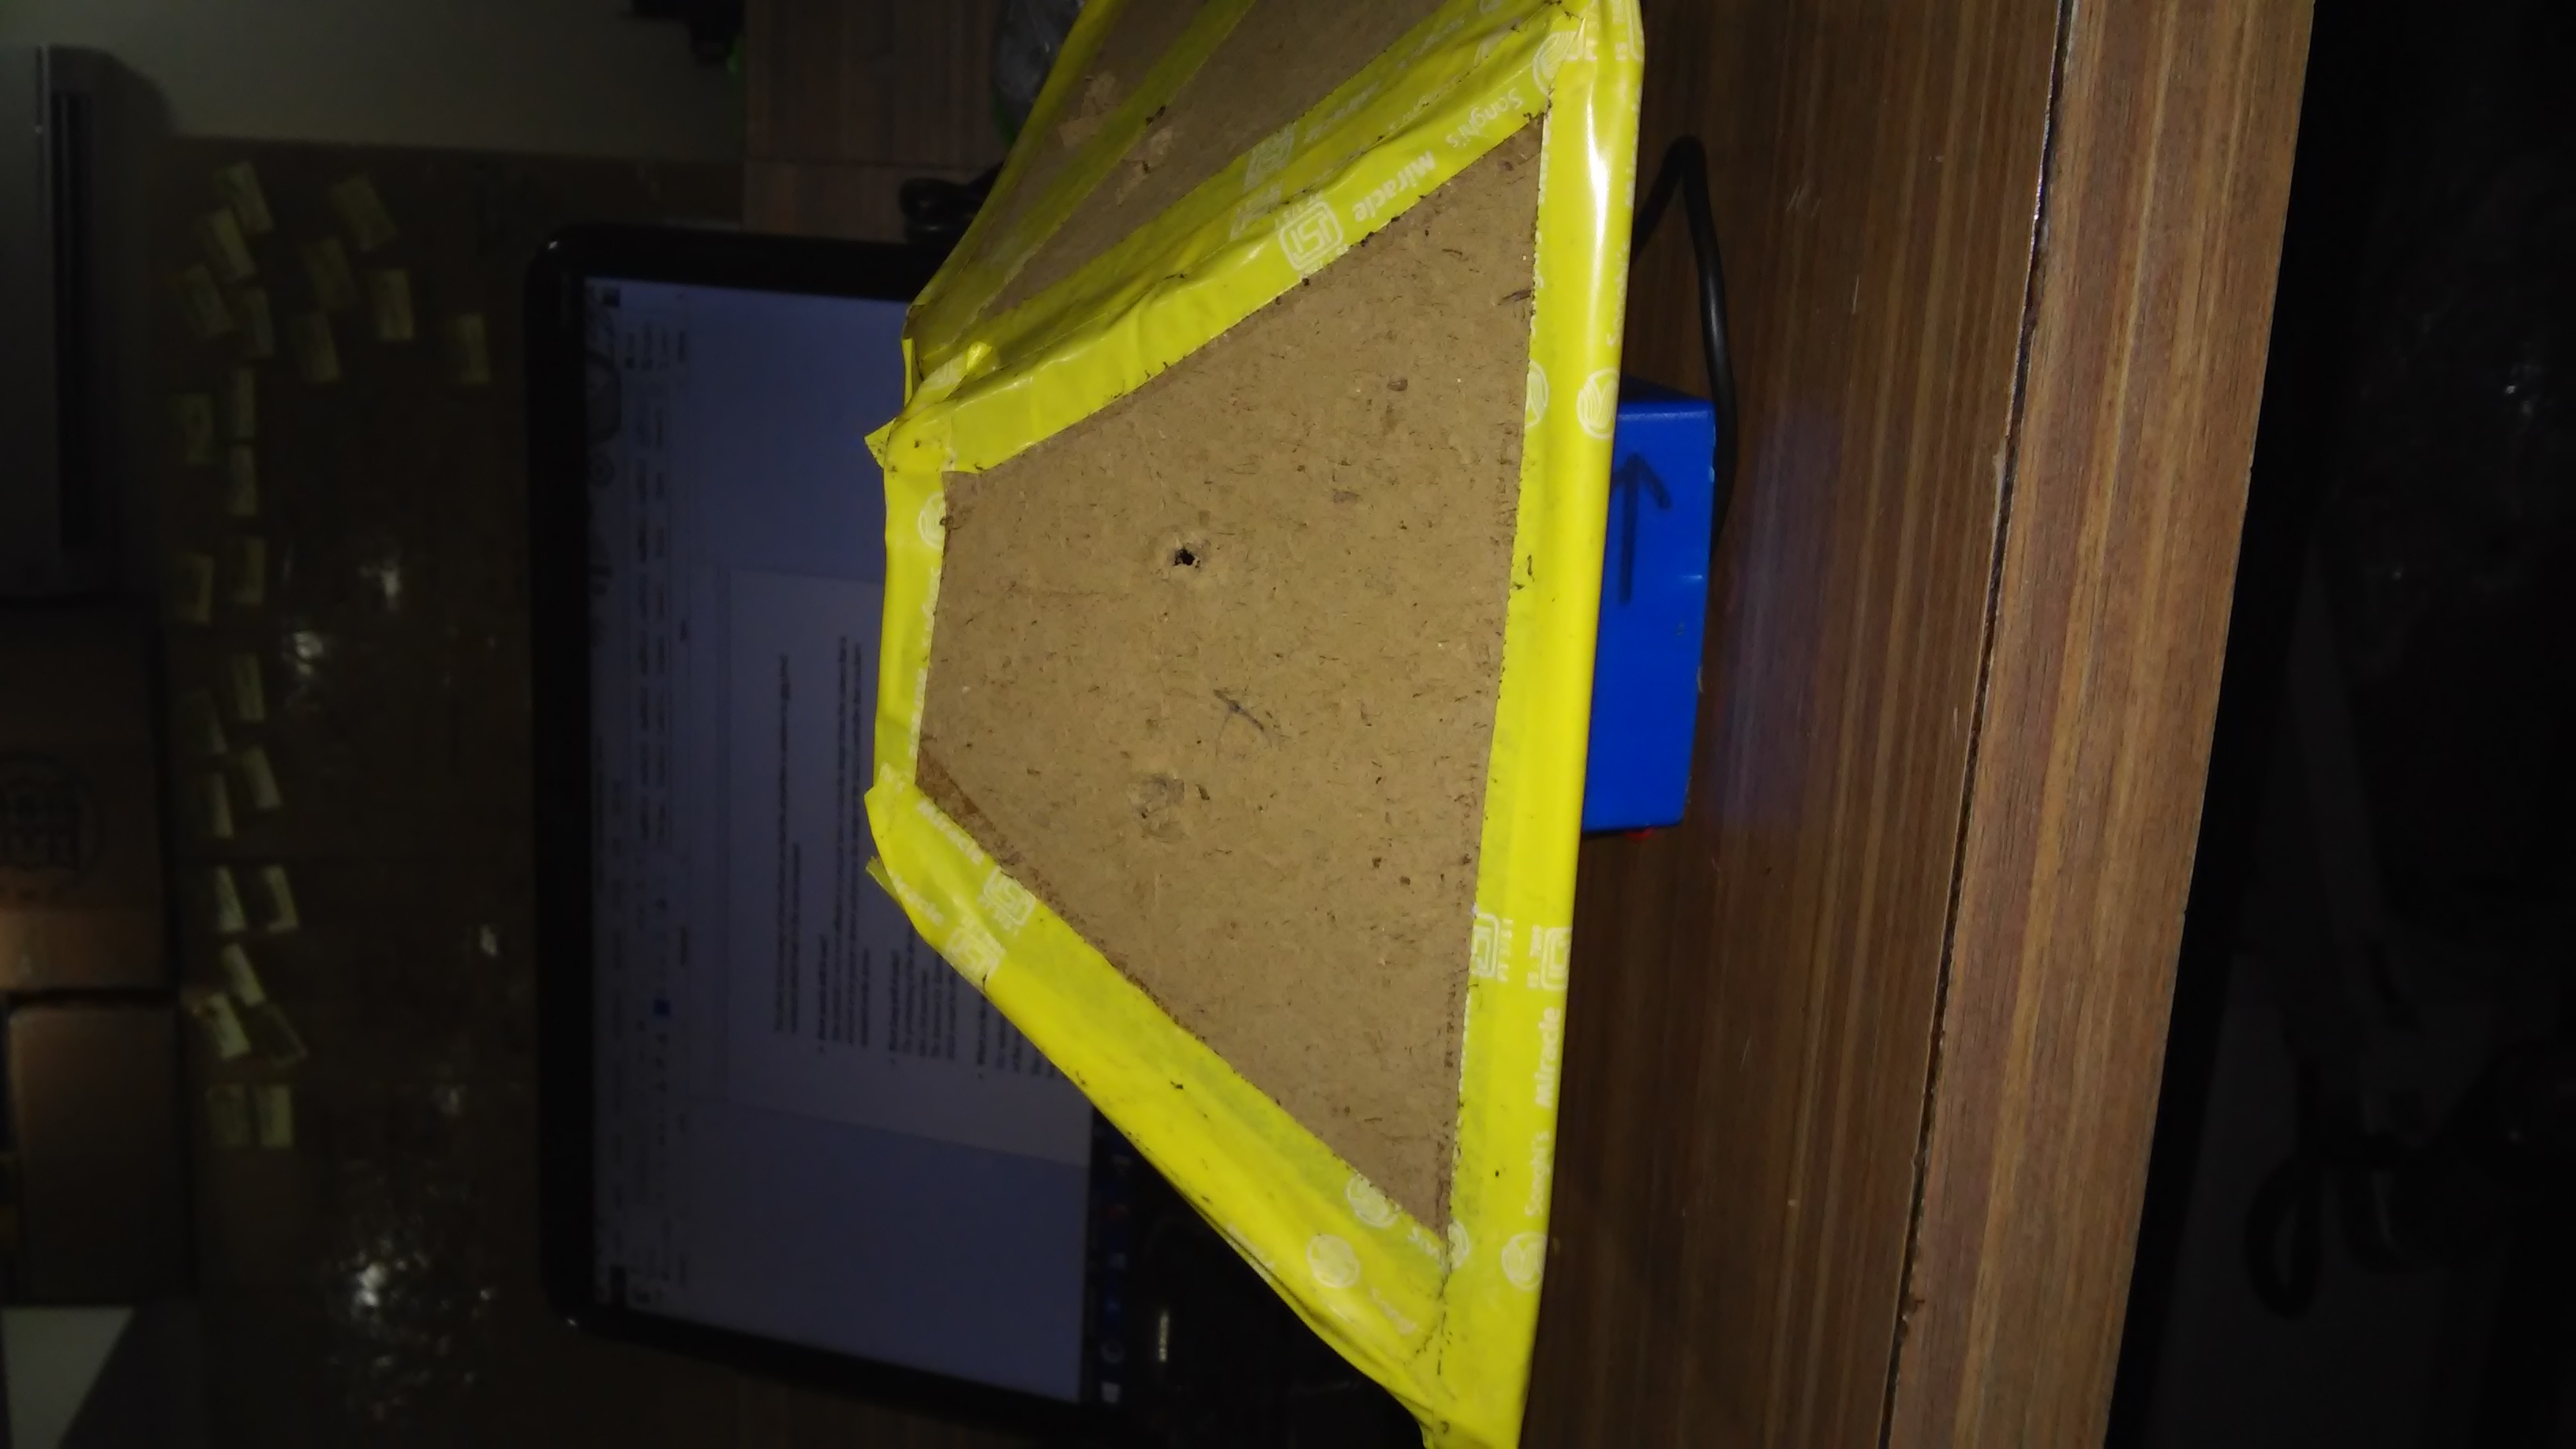
\includegraphics[width=5cm]{wwr.jpg}
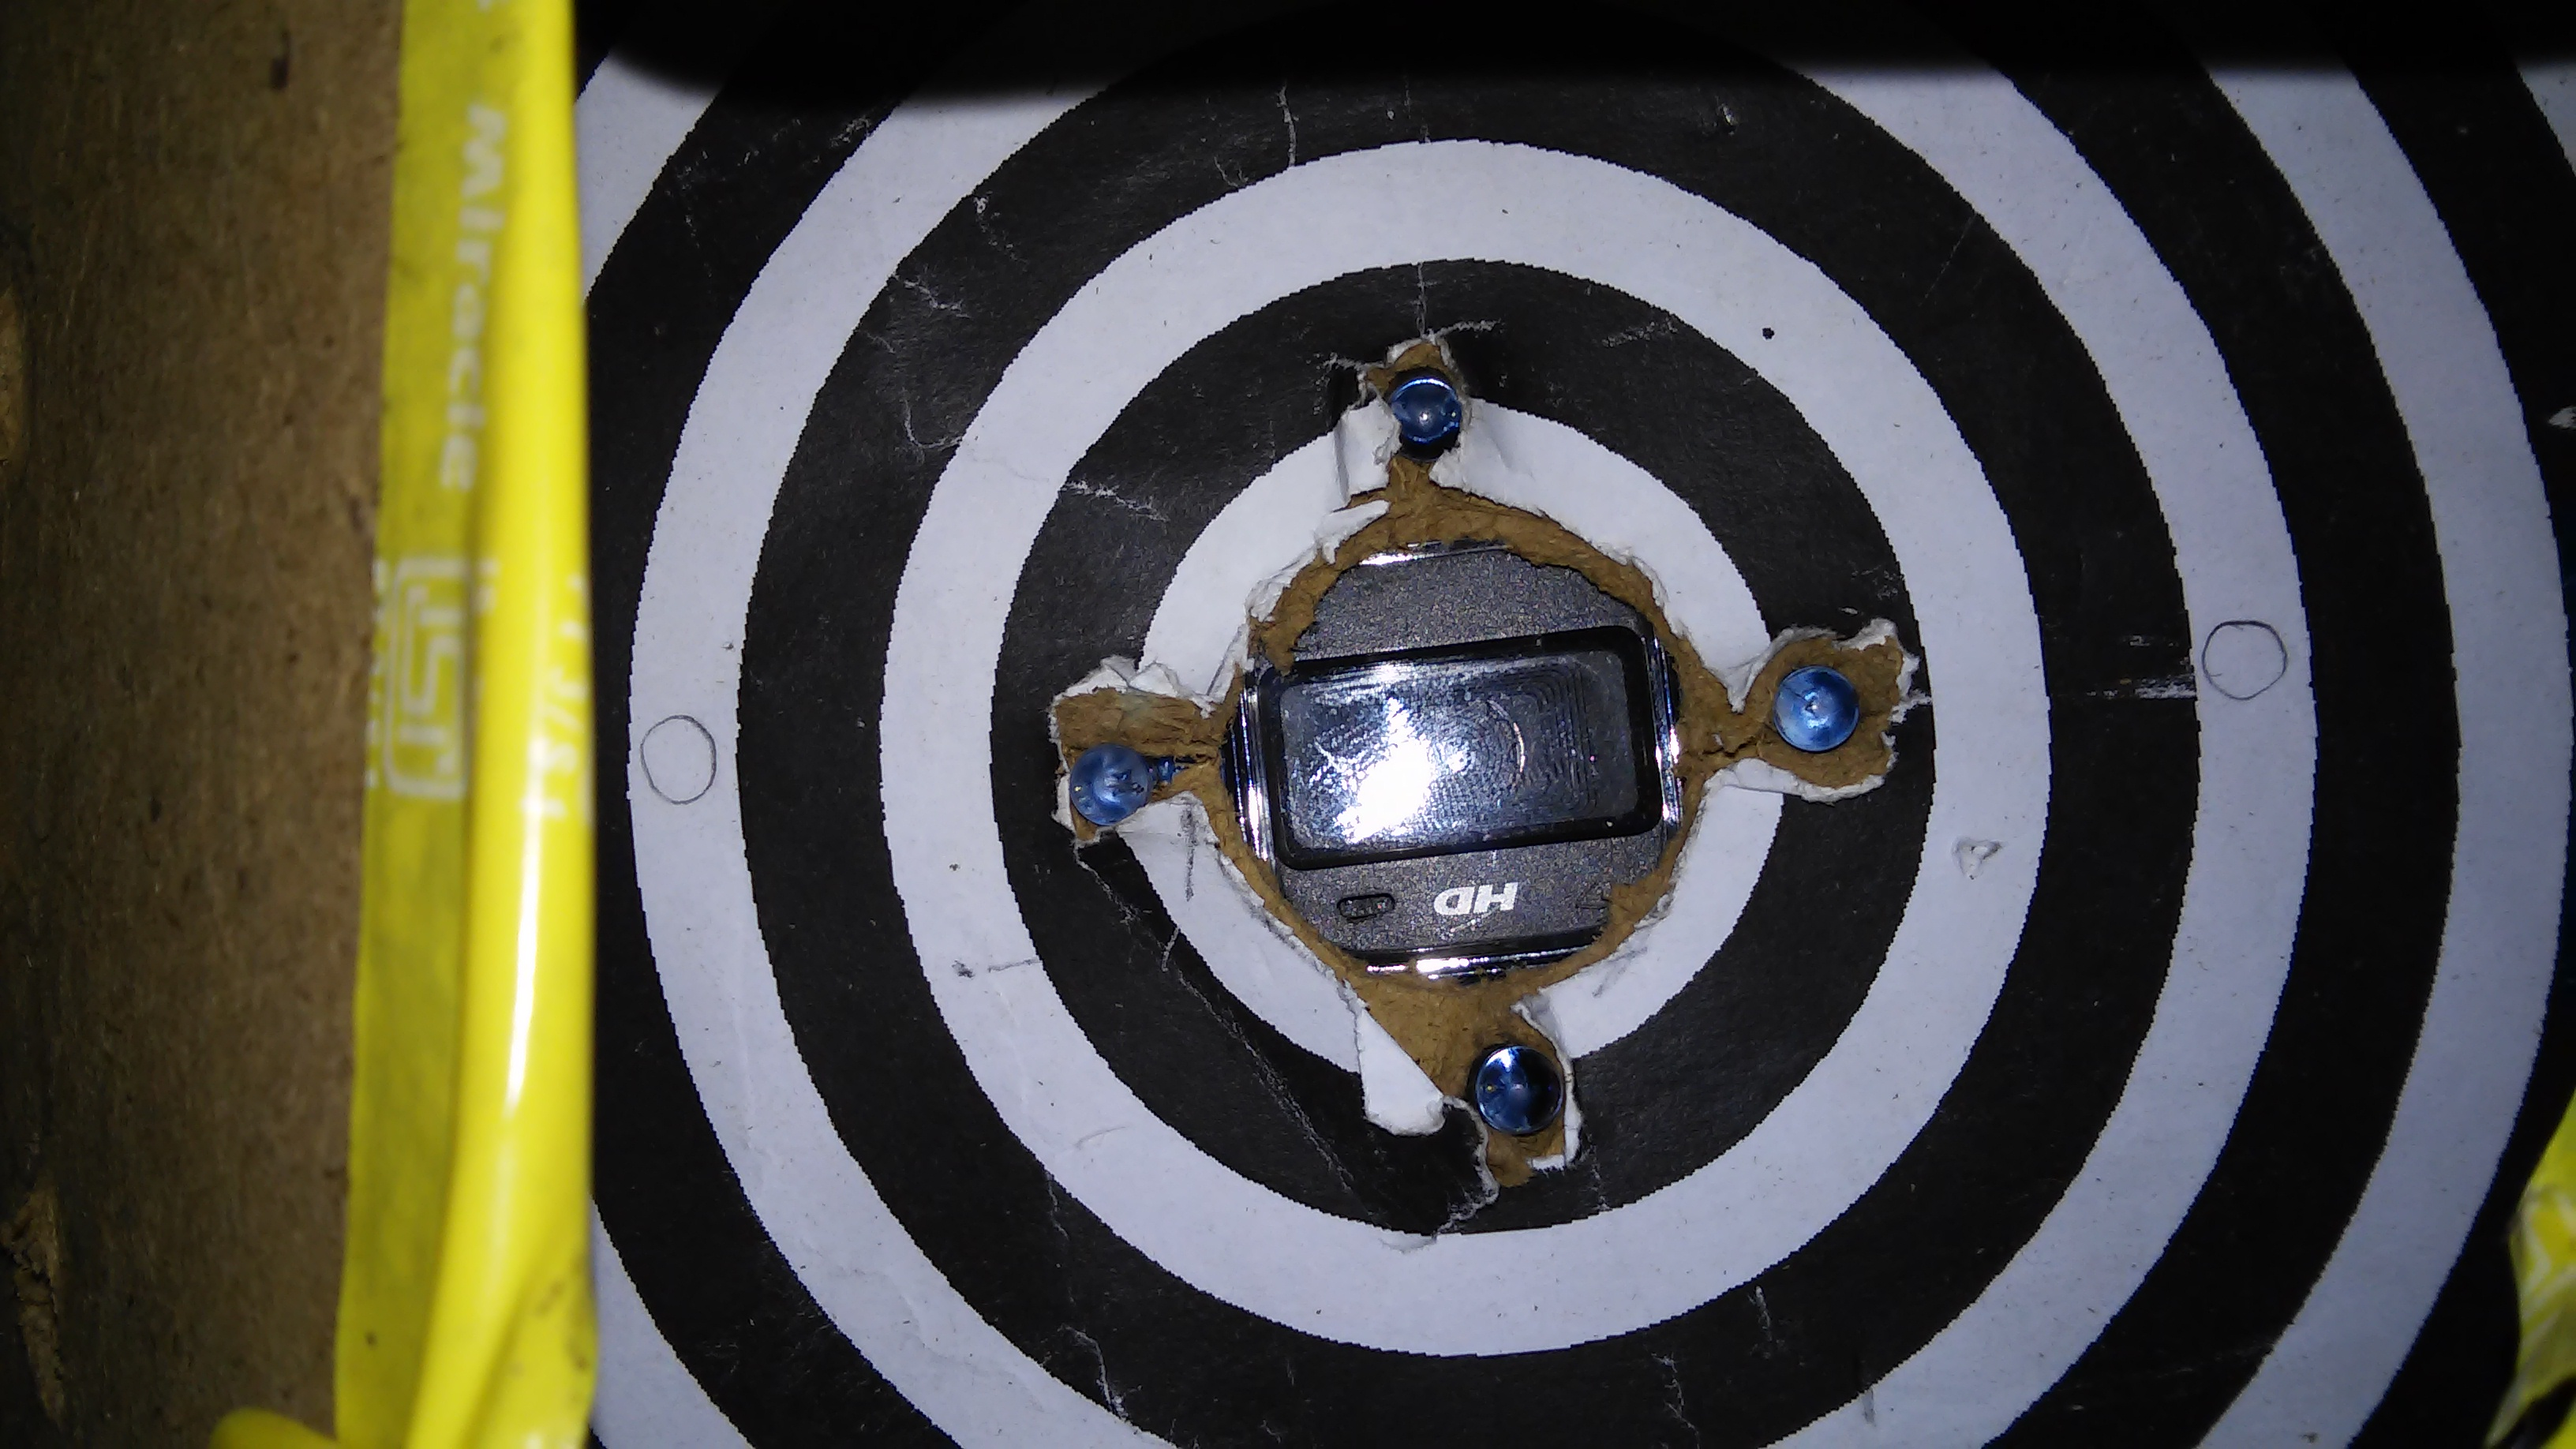
\includegraphics[width=5cm]{re.jpg}\\

The following images were obtained , which shows the corneal rings being projected onto the cornea.\\
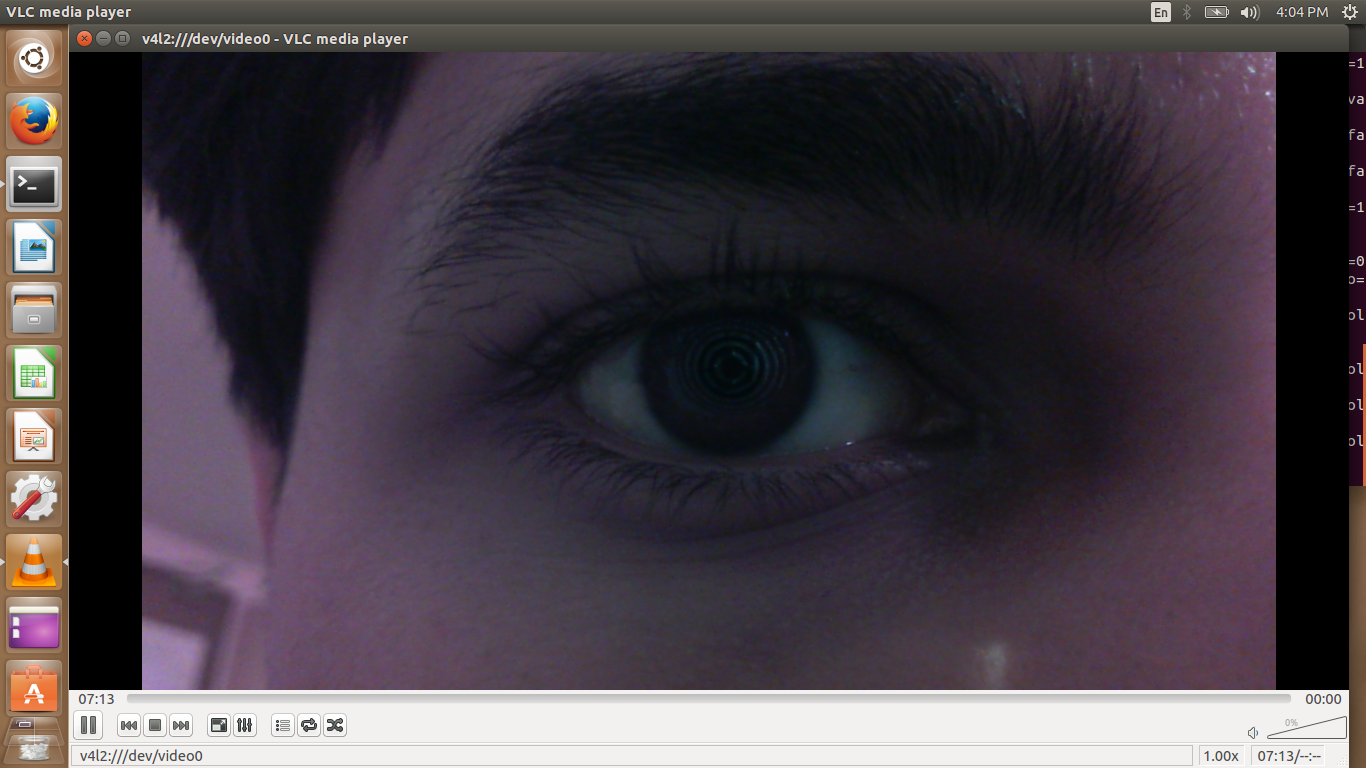
\includegraphics[width=10cm]{hj.png}
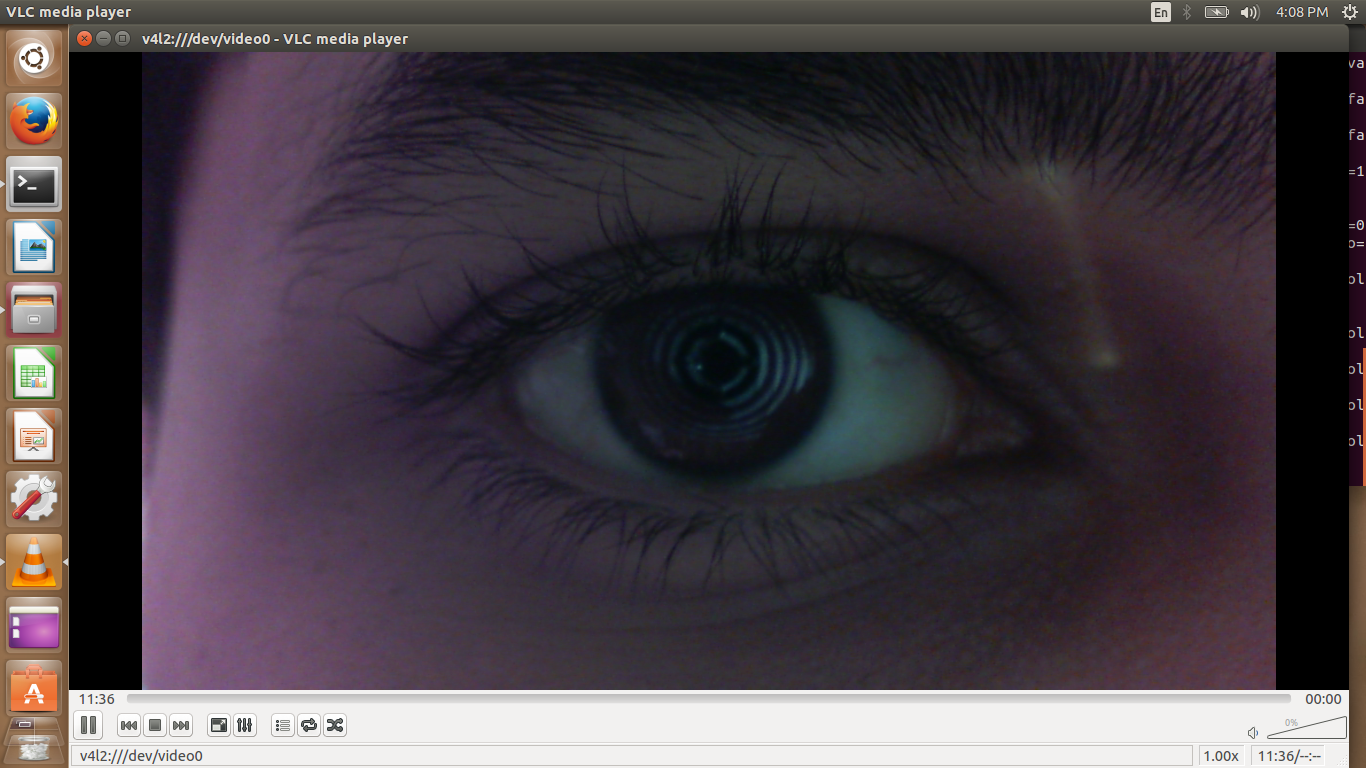
\includegraphics[width=10cm]{jk.png}

\end{document}